%-----------------------------------------------------------------------
%
% File Name: thesis.tex
%
% Author: Pekowsky, L. P.
%
% Revision: $Id$
%
%-----------------------------------------------------------------------

% document class and packages
\documentclass[12pt,notitlepage]{report}
\usepackage{bibunits}
\usepackage{syrthesis}
\usepackage{graphicx}
\usepackage{color}
\usepackage{amsmath}
\usepackage{amssymb}
\usepackage{amsfonts}
\usepackage{rotating}
\usepackage{tensor}
\usepackage{lscape}
\usepackage{units} %  do things like \units[1.234]{sec}i
\usepackage{braket}
\newcommand{\Overlap}{\Braket}
\usepackage{xspace}

\pdfoutput=1
\DeclareGraphicsExtensions{.pdf,.png}

\hbadness=10000

% new command definitions
\newcommand{\half}{\frac{1}{2}}
\newcommand{\ospsd}{\ensuremath{S_n\left(\left|f_{k}\right|\right)}}

\newcommand{\msun}{M_\odot}
\newcommand{\chisq}{\chi^2}
\newcommand{\erf}{\mathrm{erf}}
\newcommand\fake[1]{\textcolor{red}{#1}}
\newcommand\checkme[1]{\textcolor{blue}{\textbf{#1}}}


\begin{document}

\title{
Topics in Gravitational-Wave Astronomy
}
\author{\bf Larne Pekowsky}
\majorprof{Duncan Brown}
\submitdate{August 2011}
\degree{Doctor of Philosophy}
\program{Physics}
\copyrightyear{2011}
\majordept{Physics}
\havededicationtrue
\dedication{to\\ my parents}
\haveminorfalse
\copyrighttrue
\doctoratetrue
\figurespagetrue
\tablespagetrue


\Abstract{
To be written
}
\beforepreface
\prefacesection{Preface}
The work presented in this thesis stems from my participation in the LIGO
Scientific Collaboration. 

\vspace*{0.5cm}

\noindent Chapter \ref{ch:ninja1} is based on material from

\vspace*{0.25cm}

\noindent \fake{The NINJA1 paper}


\vspace*{0.5cm}

\noindent Chapter \ref{ch:boyle_et_al} is based on material from

\vspace*{0.25cm}

\noindent \fake{Boyle et. al.}


\prefacesection{Acknowledgments}
\fake{To be written.}

\prefacesection{Conventions}
\fake{To be written.}

\afterpreface

\Chapter{Comparison of high-accuracy numerical simulations of
black-hole binaries with stationary phase post-Newtonian template
waveforms}
\label{ch:comparison}
\newcommand{\Note}[1]{\textcolor{red}{\textbf{[#1]}}}
\newcommand{\Add}[1]{\textcolor{blue}{#1}}
%\renewcommand{\d}{\mathrm{d}}
%\renewcommand{\e}{\mathrm{e}}
%\renewcommand{\i}{\mathrm{i}}
\newcommand{\hyb}{\mathrm{hyb}}
\newcommand{\NR}{\mathrm{NR}}
\newcommand{\pN}{\mathrm{pN}}
\newcommand{\ADMMass}{M_{\mathrm{ADM}}}
\newcommand{\IrrMass}{M_{\mathrm{AH}}}
\newcommand{\MSun}{\ensuremath{M_{\odot}}}
\newcommand{\deff}{\ensuremath{D_{\mathrm{eff}}}} % effective distance
\newcommand{\ta}{\ensuremath{t_{\mathrm{a}}}}
\newcommand{\phia}{\ensuremath{\phi_{\mathrm{a}}}}
\newcommand{\fsamp}{\ensuremath{f_{\mathrm{s}}}}
\newcommand{\fNy}{\ensuremath{f_{\mathrm{Ny}}}}
\newcommand{\discretize}{\rightsquigarrow}
\newcommand{\software}[1]{\textsc{#1}}
\newcommand{\etal}{\textit{et al.}\xspace}
\newcommand{\G}{G}
\renewcommand{\c}{c}
\newcommand{\e}{e}
%\newcommand{\lvert}{\ensuremath{|}}
%\newcommand{\rvert}{\ensuremath{|}}

%%% Define \InnerProduct with extendible middle line
%%% Adapted from braket.sty
\makeatletter
\let\protect\relax
{\catcode`\|=\active
  \xdef\InnerProduct{\protect\expandafter\noexpand\csname InnerProduct \endcsname}
  \expandafter\gdef\csname InnerProduct \endcsname#1{%
    \begingroup
    \ifx\SavedDoubleVert\relax
    \let\SavedDoubleVert\|\let\|\IpDoubleVert
    \fi
    \mathcode`\|32768\let|\IPVert
    \left({#1}\right)
    \endgroup
  }
}
\def\IPVert{\@ifnextchar|{\|\@gobble}% turn || into \|
     {\egroup\,\mid@vertical\,\bgroup}}
\def\IPDoubleVert{\egroup\,\mid@dblvertical\,\bgroup}
\let\SavedDoubleVert\relax
\def\midvert{\egroup\mid\bgroup}
\def\SetVert{\@ifnextchar|{\|\@gobble}% turn || into \|
    {\egroup\;\mid@vertical\;\bgroup}}
\def\SetDoubleVert{\egroup\;\mid@dblvertical\;\bgroup}
\def\mid@vertical{\mskip1mu\vrule\mskip1mu}
\def\mid@dblvertical{\mskip1mu\vrule\mskip2.5mu\vrule\mskip1mu}
\makeatother


\section{Introduction}
\label{sec:Introduction} %

The coalescence of binary black holes is one the most promising
sources of gravitational waves for interferometric gravitational-wave
detectors, such as LIGO, Virgo and GEO600~\cite{thorne.k:1987}. The
first-generation LIGO detectors have achieved their design sensitivity
and recorded over one year of coincident data~\cite{Abbott:2007kva}.
This data, together with data from the Virgo detector, are currently
being searched for gravitational waves from compact binary
coalescence~\cite{Abbott:2003pj,Abbott:2005pe,Abbott:2005pf,%
  Abbott:2007xi,Abbott:2007ai,Abbott:2008}.  Upgrades to improve the sensitivity
of these detectors by a factor of two, and ultimately 10, are
underway.  Optimal searches using the enhanced detectors in 2009 will
be sensitive to black-hole coalescence out to hundreds of
megaparsecs~\cite{LIGOEnhancedLIGO}. The advanced detectors,
operational next decade, could detect black-hole binaries at distances
of over \unit[1]{Gpc}~\cite{Fritschel:2003qw}.

Optimal searches for gravitational waves use matched filtering, which
requires accurate knowledge of the waveform~\cite{thorne.k:1987}.
Previous searches in LIGO data have used post-Newtonian and
phenomenological templates to search for the coalescence of black-hole
binaries~\cite{Abbott:2005pf,Abbott:2007xi,Abbott:2008}. Over the last
several years numerical relativity has made remarkable breakthroughs
in simulating the late inspiral, merger and ringdown of black-hole
binaries. The computational cost of these simulations is high,
however, making it impractical to use them directly as template
waveforms for use in a matched-filter search. It has been shown that
there is good agreement between the waveforms generated by numerical
relativity with analytic post-Newtonian waveforms to within just a few
orbits of merger~\cite{Buonanno-Cook-Pretorius:2007, Baker2006d,
  Pan2007, Buonanno2007, Hannam2007, Boyle2007, Gopakumar:2007vh,
  Hannam2007c, Boyle2008a, Mroue2008, Hinder2008b}.

This paper uses the high-accuracy Caltech--Cornell
numerical-relativity waveforms to suggest improvements to the analytic
waveforms currently used in gravitational-wave searches by LIGO and
Virgo.  A similar study has been performed by Pan~\etal using
numerical data from Pretorius and the Goddard groups~\cite{Pan2007}.
Our main results are in agreement with their conclusion that a simple
extension of the existing stationary-phase approximation to the
adiabatic post-Newtonian waveforms (called \textit{TaylorF2} in
Ref.~\cite{Damour2001}) yields high overlaps with numerical waveforms.

In Sec.~\ref{sec:Searches}, we review the current techniques used for
searching for gravitational waves in gravitational-wave detector data.
We discuss the construction of the waveform---a pN--NR hybrid---in
Sec.~\ref{sec:PNNRHybridWaveform}.  In Sec.~\ref{sec:Efficiency} we
employ the hybrid waveform in a comparison of the detection efficiency
of gravitational-wave templates that may be used in upcoming searches
of LIGO and Virgo data.  Finally, in Sec.~\ref{sec:Recommendations},
we discuss improvements that may be made to the current data-analysis
techniques to optimize overlaps.

Throughout this paper, we use only the $(l,m)=(2,2)$ component of the
waveform $\Psi_{4}^{2,2}$ (as defined, e.g., in~\cite{Boyle2008a}).
For convenience, we drop the superscript.  Whenever possible, we use
dimensionless quantities, like $r\,M\,\lvert \Psi_{4} \rvert$, where
$r$ is the areal radius of the observation sphere, and $M$ is the
total apparent-horizon mass of the holes in the initial data.
However, for any calculation involving the LIGO noise curve, we have a
physical scale, and thus use standard mks units.

% , where
% \begin{eqnarray}
%  \label{eq:units}
%  \G &= \unit[6.67259 \times 10^{-11}]{{m^3}\ {kg^{-1}\ s^{-2}}}\ ,\\
%  \c &= \unit[299792458]{{m}\ {s^{-1}}}\ ,\\
%  \MSun &= \unit[1.98892 \times 10^{30}]{kg}\ ,\\
%  \unit[1]{Mpc} &= \unit[3.08568025 \times 10^{22}]{m}\ .
%\end{eqnarray}


%%%%%%%%%%%%%%%%%%%%%%%%%%%%%%%%%%%%%%%%%%%%%%%%%%%%%%%%%%%%%%%%%%%%%%
%%%%%%%%%%%%%%%%%%%%%%%%%%%%%%%%%%%%%%%%%%%%%%%%%%%%%%%%%%%%%%%%%%%%%%
\section{Searches for gravitational waves from black-hole binaries}
\label{sec:Searches}


In this paper we are concerned with overlaps between pN waveforms and
NR signals; to weight the inner product we use the following PSDs for
Initial and Advanced LIGO: for Initial LIGO we use an analytic
approximation to the LIGO design PSD given by
\begin{eqnarray}
  S_n(f) &= &3.136 \times 10^{-4} \bigg[
  \left(\frac{ 4.49 f}{150.0}\right)^{-56.0} \nonumber \\
  &+ & 0.16 \left(\frac{f}{150}\right)^{-4.52}
  + \left(\frac{f}{150.0}\right)^2 + 0.52
  \bigg]
\end{eqnarray}
All integrals start from 40 Hz.  As shown in
Fig.~\ref{fig:StildesAndInitialPSD}, at this frequency the noise is an
order of magnitude higher than its lowest value, and below this
frequency it rises rapidly as $\sim f^{-56}$.  The region below 40 Hz
therefore contributes very little signal power to the
SNR~\cite{Abbott:2007xi}.  The PSD for Enhanced LIGO, which will
begin operation in mid 2009, has a similar shape to that for Initial
LIGO although it has a factor of $\sim 2$ increase in strain
sensitivity.  Our results using the Initial-LIGO PSD are therefore
valid for Enhanced LIGO, as the sensitivity factor cancels in
Eq.~\eqref{eq:OverlapDefinition}; overlaps depend on the \emph{shape}
of the PSD.

For Advanced LIGO we use the GWINC program~\cite{AdvancedLIGONoise} to
generate the PSD.  Bench reports the PSD in increments of 0.0124 Hz.
When calculating discrete integrals against signals sampled at other
frequencies we obtain values for the PSD by linearly interpolating
between the values provided by Bench.  We start integrals at 10 Hz as
that is the point where the noise has increased by two orders of
magnitude above its minimum, as also shown in
Fig.~\ref{fig:StildesAndInitialPSD}.




% \subsection{Discretization}
% \label{sec:Discretization}

% The direct and inverse Fourier transforms are defined (using the
% standard LIGO conventions~\cite{T010095}) as
% \begin{align}
%   \label{eq:FourierTransform}
%   \tilde{s}(f) &\equiv \int_{-\infty}^{\infty}\, s(t)\, \e^{-2\pi\i
%     f t}\,
%   \d t\ , \\
%   \label{eq:InverseFourierTransform}
%   s(t) &= \int_{-\infty}^{\infty}\, \tilde{s}(f)\, \e^{2\pi\i f t}
%   \, \d f\ .
% \end{align}
% In transferring these and the continuum expressions of preceding
% sections to computer, we need to introduce two changes.

% First, the ranges of integration must be restricted to finite
% intervals.  We need to assume that the physical signal contains
% nothing of interest at frequencies higher than $\fNy$ or,
% considering negative frequencies, lower than $-\fNy$.  For
% notational simplicity, we define the discretized Fourier transform
% to be periodic, with period $2\fNy$.  Similarly, we will assume that
% the signal $s$ is periodic, with period $T$.  Thus, we can restrict
% each of the integrals given above to one period of the relevant
% quantity.

% Second, the quantities must be given on a discrete grid.  We will
% assume that the signal $s$ is sampled at $N$ uniform intervals of
% $\Delta t=T/N$.  This will give rise to a frequency discretization
% of $\Delta f = 1/T = 1/N\Delta t$.  We define the quantities
% \begin{equation}
%   t_{j} = j\Delta t \quad \text{and} \quad f_{k} = k\Delta f\ ,
% \end{equation}
% for \emph{all} integers $j$ and $k$.  It is not hard to see that the
% highest frequency that can be represented on this discrete set is
% bounded by the Nyquist frequency $\fNy=1/2\Delta t$.

% The combined operation of discretizing and restricting to finite
% range will be denoted by $\discretize$, so
% \begin{align}
%   \label{eq:DiscreteFourierTransform}
%   \tilde{s}(f_{k}) &\discretize \sum_{t_{j}>-N\Delta t/2}^{N\Delta
%     t/2}\, s(t_{j})\, \e^{-2\pi\i f_{k} t_{j}}\, \Delta t
%   \\
%   \label{eq:DiscreteFourierTransformTwo}
%   &\discretize \Delta t\, \sum_{j=0}^{N-1}\, s(t_{j})\, \e^{-2\pi\i
%     j k/N}\ ,
%   \\
%   \label{eq:DiscreteInverseFourierTransform}
%   s(t_{k}) &\discretize \sum_{f_{j} > -\fNy} ^{\fNy}\,
%   \tilde{s}(f_{j})\, \e^{2\pi\i f_{k} t_{j}}\, \Delta f
%   \\
%   \label{eq:DiscreteInverseFourierTransformTwo}
%   &\discretize \Delta f\, \sum_{j=0}^{N-1}\, \tilde{s}(f_{k})\,
%   \e^{2\pi\i j k/N}\ .
% \end{align}
% Note that in the second step of each of these expressions, we have
% used the periodic character of $s$ to re-express negative times as
% positive, and the periodic character of $\tilde{s}$ to re-express
% negative frequencies as positive.  We have also used the relation
% $f_{k}t_{j} = j k/N$.

% A notational subtlety arises when using the frequency-domain
% quantity.  The symbol $\tilde{s}_{k}$ is defined as the sum in
% Eq.~\eqref{eq:DiscreteFourierTransformTwo}, without the factor of
% $\Delta t$~\cite{DBrownThesis}.  In particular, we have
% $\tilde{s}(f_{k}) \discretize \Delta t\, \tilde{s}_{k}$.  The
% expressions given above for $\tilde{s}(f_{k})$ and $s(t_{j})$ should
% not depend strongly on the fineness of the discretization (for
% sufficiently fine discretizations).  Clearly, then, $\tilde{s}_{k}$
% \emph{will} depend strongly on the discretization.  Though the
% factor of $\Delta t$ should drop out for calculations using
% normalized quantities, for calculations of the signal-to-noise
% ratio, or demonstrations of $\tilde{s}(f_{k})$, it is an important
% distinction that needs to be kept in mind.  For example, the
% \software{FFTW} and \software{Matlab} software packages use
% $\tilde{s}_{k}$ as their standard frequency-domain quantity.
% Throughout the remainder of this paper, we will use
% $\tilde{s}(f_{k})$ exclusively.

% For completeness, we include the expressions
% \begin{align}
%   \InnerProduct{s|h} &\discretize 2\, \Re \sum_{k=0}^{N-1}\,
%   \frac{\tilde{s}(f_{k})\, \tilde{h}^{\ast}(f_{k})}{S_{n}(\lvert
%     f_{k} \rvert)}\, \Delta f
%   \\
%   &\discretize 4\, \Re \sum_{k=0}^{\lfloor N/2 \rfloor}\,
%   \frac{\tilde{s}(f_{k})\, \tilde{h}^{\ast}(f_{k})}{S_{n}(f_{k})}\,
%   \Delta f\ ,
%   \\
%   \Overlap{s|h} &\discretize 2 \max_{\ta}\, \left\lvert
%     \sum_{k=0}^{N-1}\, \frac{\tilde{s}(f_{k})\,
%       \tilde{h}^{\ast}(f_{k})}{S_{n}(\lvert f_{k} \rvert)}\,
%     \e^{2\pi \i f_{k}\ta}\, \Delta f \right\rvert
%   \\
%   &\discretize 4 \max_{\ta}\, \left\lvert \sum_{k=0}^{\lfloor N/2
%       \rfloor}\, \frac{\tilde{s}(f_{k})\,
%       \tilde{h}^{\ast}(f_{k})}{S_{n}(f_{k})}\, \e^{2\pi \i
%       f_{k}\ta}\, \Delta f \right\rvert\ .
% \end{align}
% The notation $\lfloor N/2 \rfloor$ denotes the greatest integer less
% than or equal to $N/2$.


%%%%%%%%%%%%%%%%%%%%%%%%%%%%%%%%%%%%%%%%%%%%%%%%%%%%%%%%%%%%%%%%%%%%%%
%%%%%%%%%%%%%%%%%%%%%%%%%%%%%%%%%%%%%%%%%%%%%%%%%%%%%%%%%%%%%%%%%%%%%%
\section{PN--NR hybrid waveform}
\label{sec:PNNRHybridWaveform} %


In order to perform our comparison we need to construct a ``true''
black-hole binary waveform, which we might expect to observe with
detectors.  A numerical simulation will provide the data for the
crucial nonlinear merger phase.  We carefully extract the data and
extrapolate it to large radius, and investigate the effects of
numerical error on the final result.  Because this waveform is very
computationally expensive to produce, it covers only about 32 cycles,
which is not sufficient for a thorough investigation of the
possibility of detecting it in searches of data from
gravitational-wave detectors.  Thus, we match the numerical waveform
to a post-Newtonian waveform, producing a hybrid which extends for
many thousands of cycles, covering the entire band of interest.

\subsection{Numerical simulation, extraction, and extrapolation}
\label{sec:WaveformExtractionAndExtrapolation}
The numerical simulation is the same as that described in
Refs.~\cite{Boyle2007, Scheel2008}: an equal-mass, non-spinning,
black-hole binary with reduced
eccentricity~\cite{Pfeiffer-Brown-etal:2007}, beginning roughly 16
orbits before merger, continuing through merger and
ringdown~\cite{Scheel2008}.  It is performed with the Caltech--Cornell
pseudospectral code, using boundary conditions designed to prevent
constraint violations and gravitational radiation from entering the
domain~\cite{Holst2004, Lindblom2006}.

Data is extracted from the simulation in the form of the
Newman--Penrose scalar
\begin{equation}
  \Psi_{4} = -C_{\alpha \beta \gamma \delta} l^{\alpha}
  \bar{m}^{\beta} l^{\gamma} \bar{m}^{\delta}\ ,
\end{equation}
where $l^{\alpha}$ and the complex vector $\bar{m}^{\beta}$ are
constructed with reference to the coordinate basis.  Along the
positive $z$ axis, we have
\begin{eqnarray}
  l^{\alpha} &= & \frac{1}{\sqrt{2}}\, \left( t^{\alpha} - z^{\alpha}
  \right)\ , \\
  \bar{m}^{\beta} &= & \frac{1}{\sqrt{2}}\, \left(
    \frac{\partial}{\partial x} - i\, \frac{\partial}{\partial y}
  \right)^{\beta}\ .
\end{eqnarray}

Here, $t^{\alpha}$ is the timelike unit normal to the spatial
hypersurface, and $z^{\alpha}$ is the unit vector in the positive $z$
direction.  The vectors $\partial/\partial x$ and $\partial/\partial
y$ are the standard coordinate vectors, which are not normalized.
$\Psi_{4}$ is extracted as a function of time, at various radii along
the positive $z$ axis.  This is then extrapolated to large radii, as
described in Ref.~\cite{Boyle2007}, and in greater detail in
Ref.~\cite{Boyle2008}.

% The Nyquist frequency of the data is \Note{bla, as compared to the
%   measured ringdown frequency}.  Note that the LIGO Nyquist
% frequency is \unit[2048]{Hz}, which is lower than the ringdown
% frequency for masses above bla.

The measured (instantaneous) frequency at the beginning of the
simulation is
\begin{equation}
  \label{eq:MeasuredStartingFreq}
  % \frac{G\,M}{c^{3}}\,\omega & = 0.0333 \pm 0.0002\ , \\
  % \frac{G\,M}{c^{3}}\,f & = 0.00530 \pm 0.00003\ , \\
  f_{\mathrm{initial}} = \unit[(1.08 \pm 0.01) \times 10^{3}]{Hz}\,
  \frac{\MSun}{M}\ .
\end{equation}
The measured ringdown frequency is
\begin{equation}
  \label{eq:MeasuredRingdownFreq}
  % \frac{G\,M}{c^{3}}\,\omega & = 0.553 \pm 0.007\ , \\
  % \frac{G\,M}{c^{3}}\,f & = 0.088 \pm 0.001\ , \\
  % \omega & = \unit[(112 \pm 1) \times 10^{4}]{\frac{1}{sec}}\,
  % \frac{\MSun}{M}\ , \\
  f_{\mathrm{ringdown}} = \unit[(1.78 \pm 0.02) \times 10^{4}]{Hz}\,
  \frac{\MSun}{M}\ .
\end{equation}
The measured \emph{Christodoulou} mass and spin of the final black
hole are
\begin{eqnarray}
  \label{eq:MeasuredFinalMass}
  M_{\chi\mathrm{, final}} &= &(0.95162 \pm 0.00002)\, M_{\chi\mathrm{,
      initial}}\ , \\
  \label{eq:MeasuredFinalSpin}
  S_{\mathrm{final}} &= &(0.68646 \pm 0.00004)\, M^{2}_{\chi\mathrm{, final}}\ .
\end{eqnarray}
Using this value for the spin, a quasi-analytic formula due to
Echeverria~\cite{Echeverria1989} predicts a value of
$\unit[1.77\times10^{4}]{Hz}\, \frac{\MSun}{M}$, for the ringdown
frequency, in close agreement with the measured frequency.

\subsection{Accuracy of the numerical simulation}
\label{sec:Accuracy}

The numerical waveform will be the standard against which we will
judge the \textit{TaylorF2} waveforms used in LIGO data analysis.  To
understand how precisely we should trust our final results, we need to
understand the accuracy of the waveform itself.  The most obvious
measure of the error in this fiducial waveform is its convergence with
increasing numerical resolution.  Fig.~\ref{f:accuracy} shows the
overlap (Eq.~\eqref{eq:OverlapDefinition}) between waveforms computed
at different resolutions.  The data used here are the extrapolated
$\Psi_4$ waveforms, integrated in time twice.
%%%%%%%%%%%%%%%%%%%%%%%%%%%%%%%%%%%%%%%%%%%%%%%%%%%%%%%%%%%%%%%%%%%%%%
\begin{figure}
  \begin{center}
    \includegraphics[width=0.55\linewidth]{figures/comparison/Accuracy}
  \end{center}
  \caption[Convergence testing for numerical waveforms ]{
  \label{f:accuracy}
    Convergence testing for numerical waveforms from a
    data-analysis perspective, using the match between waveforms
    computed at different numerical resolutions.  The waveforms are
    scaled to various masses, and the Initial-LIGO noise curve is used
    in the calculation of the match.  The upper panel shows the
    overlap without maximization over arrival time and phase; the
    lower panel shows the overlap after maximization.  In each panel,
    the lower (dashed) line compares the lowest- and
    highest-resolution simulations, while the upper (solid) line
    compares the medium- and highest-resolution simulations.  Note
    that this plot uses only numerical data, with no post-Newtonian
    contribution.}
\end{figure}%
%%%%%%%%%%%%%%%%%%%%%%%%%%%%%%%%%%%%%%%%%%%%%%%%%%%%%%%%%%%%%%%%%%%%%%

Because of the short extent of the numerical waveforms, we need to be
careful when using their Fourier transforms.  The signal can be
corrupted easily by the non-periodicity of the waveforms, and the
discontinuous jumps that result.  For Fig.~\ref{f:accuracy} we
mitigate this problem by increasing the sampling frequency of the
input data, and restricting the Fourier transform to frequencies
corresponding to instantaneous frequencies contained in the data.  The
input data can easily be upsampled in the time domain by interpolating
the phase and amplitude of the complex data to a finer time grid.  We
then perform the transform, and explicitly set the data to zero at
frequencies below $f_{\mathrm{initial}}$ and above
$f_{\mathrm{ringdown}}$, as given in
Eqs.~\ref{eq:MeasuredStartingFreq} and~\ref{eq:MeasuredRingdownFreq}.
While the results do depend on whether or not we impose these cutoffs,
they do not depend sensitively on the actual cutoff frequencies.

The overlap between the lowest- and highest-resolution simulations
(dashed lines) actually passes through zero, as shown in the upper
panel.  Presumably, this is because of loss of phase accuracy over the
course of the simulation.  All three simulations begin with the same
initial data, so the waveforms are most similar at the beginning.
Masses for which this is the most important segment (the lowest
masses) will naturally have the highest overlap between resolutions.
As the simulation progresses, numerical error accumulates---notably in
the phase---so the overlap decreases with masses for which later
segments dominate the overlap (higher masses).  When the overlap is
optimized over arrival time and phase, we can see that the overlap
becomes much better, as shown in the lower panel, indicating
sufficient accuracy within any frequency band for which phase
coherence is required.  In either case, the medium and
highest resolutions are much more nearly the same.  Without
optimization, their overlap is within a few tenths of a percent of 1;
after optimization, the overlap is within $10^{-6}$ of 1.

In the rest of our analysis we use the highest-resolution waveform.
Because we always optimize over arrival time and phase, the lower
panel of Fig.~\ref{f:accuracy} is the most relevant, and shows that
the waveform has converged to very high accuracy.  The overlaps we
quote below will only be given to three decimal places at most,
because this is roughly the accuracy of the single-precision numerical
methods used in the rest of the paper.  This accuracy is also
sufficient for searches of gravitational-wave data.  Thus, the
truncation error of the simulated waveform is irrelevant for those
purposes.

Other sources of error include residual eccentricity and spin, the
influence of the outer boundary of the simulation, extrapolation
errors, and coordinate effects, as discussed in Ref.~\cite{Boyle2007}.
The eccentricity had a disproportionately large effect on the error
quoted in that paper because of the matching technique, which is not
used here.  Restricting attention to the other effects of
eccentricity, the uncertainty falls below that due to numerical error.
Similarly, using the techniques of Ref.~\cite{Lovelace2008}, the
initial spins of the black holes have been measured more reliably, and
found to be more than an order of magnitude smaller than previously
determined, allowing us to reduce the estimate for that error to less
than the numerical truncation error.  The various coordinate effects
were all estimated to be of roughly the same magnitude as the
numerical error.

With the numerical error being many times more accurate than needed
for this analysis, and the other sources of uncertainty being of
roughly the same size, these considerations indicate that the overall
error in our fiducial waveform is substantially less than the
precision needed for this analysis.


%%%%%%%%%%%%%%%%%%%%%%%%%%%%%%%%%%%%%%%%%%%%%%%%%%%%%%%%%%%%%%%%%%%%%%
%%%%%%%%%%%%%%%%%%%%%%%%%%%%%%%%%%%%%%%%%%%%%%%%%%%%%%%%%%%%%%%%%%%%%%
\section{Detection efficiency of gravitational-wave templates}
\label{sec:Efficiency} %

We now compare the signal described in the previous section to
restricted, stationary phase \textit{TaylorF2} post-Newtonian
templates with terms up to order 2.0, order 3.5, and a ``pseudo-4.0
pN-order'' term recommended in Ref.~\cite{Pan2007}.  Overlaps are
calculated using the techniques of Sec.~\ref{sec:MatchedFiltering},
with the signal $s$ being the hybrid waveform described in
Sec.~\ref{sec:PNNRHybridWaveform} scaled to a range of masses.  We
consider both the Initial- and Advanced-LIGO noise curves.
% We consider mass ranges up to the value where the ISCO frequency is
% roughly at the lower limit of sensitivity set by the seismic wall:
% $110 \MSun$ for Initial LIGO; $440 \MSun$ for Advanced LIGO.

Plots of the hybrid waveforms in comparison to the Initial-LIGO noise
curve are shown in Fig.~\ref{fig:StildesAndInitialPSD}.
%%%%%%%%%%%%%%%%%%%%%%%%%%%%%%%%%%%%%%%%%%%%%%%%%%%%%%%%%%%%%%%%%%%%%%
\begin{figure}
  \begin{center}
    \includegraphics[width=0.55\linewidth]{figures/comparison/StildesAndInitialPSD}
  \end{center}
  \caption[Hybrid Caltech--Cornell waveform scaled to various total masses]{
  \label{fig:StildesAndInitialPSD}
    Hybrid Caltech--Cornell waveform scaled to various total
    masses, with sources optimally oriented and placed at
    \unit[100]{Mpc}, shown against the Initial- and Advanced-LIGO
    noise curves.  Markers are placed along the lines at frequencies
    corresponding to various instantaneous frequencies of the
    waveforms.  The triangles represent the beginning and end of the
    blending region; the circle represents the ISCO frequency; the
    square the light-ring; and the diamond the measured ringdown
    frequency.  See the text for discussion of the normalization.  The
    values given for $\rho$ use the Initial-LIGO noise curve, with
    sources at a distance of 100\,Mpc.}
\end{figure}%
%%%%%%%%%%%%%%%%%%%%%%%%%%%%%%%%%%%%%%%%%%%%%%%%%%%%%%%%%%%%%%%%%%%%%%
The masses are chosen so that various frequencies of interest (the
final stitching frequency, the ISCO, and the ringdown) occur at the
``seismic wall'' for Initial LIGO: \unit[40]{Hz}.  The waveforms
$\tilde{s}$ are scaled to depict the detectability of the signal,
typically quantified by the SNR introduced in
~\eqref{eq:InnerProductSNR}, which may be written as
\begin{equation}
  \label{eq:SNR}
  \rho^{2} \equiv \int_0^\infty \frac{4\, \tilde{s}(f)\,
    \tilde{s}^\ast(f)} {S_n(f)}\, d f = \int_0^\infty
  \frac{\left\lvert 2\, \tilde{s}(f)\, \sqrt{f} \right\rvert^{2}}
  {S_n(f)}\, d\ln{f}\ .
\end{equation}
In the final expression, the numerator and denominator have the same
units, and are directly comparable.  Because the square root of the
denominator is familiar, we plot that along with the square root of
the numerator.  Plotting these two quantities together gives a
graphical impression of the detectability of the waveform, and the
relative importance of each part of the waveform, by its height above
the noise curve.  In Ref.~\cite{BradyCreighton2002}, Brady and
Creighton define a slightly different quantity, the characteristic
strain $h_{\mathrm{char}} \equiv f\, \lvert \tilde{s}(f) \rvert\ .$
The relative factor of $\sqrt{f}$ they use is present so that they can
plot $h_{\mathrm{char}}$ against $\sqrt{f\, S_{n}(f)}$.  Cutler and
Thorne~\cite{Cutler2002} define still another quantity, the signal
strength $\tilde{h}_{s}(f)$, which is related to the Fourier transform
by $\tilde{h}(f) = \sqrt{5}\, \frac{T}{N}\, \tilde{h}(s)\ .$ The
factor of $\sqrt{5}$ comes from averaging over the orientation of the
binary, which we do not do.  $T/N$ is the ratio of the threshold to
the rms noise at the endpoint of signal processing.

\iffalse
\begin{figure}
  % \includegraphics[width=\linewidth]{figures/comparison/AmoebaHistogram}
  \begin{center}
    \includegraphics[width=0.55\linewidth]{figures/comparison/Histogram}
  \end{center}
  \caption{Histogram of overlaps found by 300 instances of the Amoeba
    algorithm, optimizing the overlap against a given waveform over
    $M, \eta, f_c$, with randomized initial conditions.  Note the
    logarithmic scale on the vertical axis.  The majority of instances
    produced a lower overlap than the optimum.  We interpret this as
    pointing to the existence of a broad local maximum which did not
    coincide with the global maximum.}
  \label{fig:AmoebaHistogram}
\end{figure}%
\fi

For each template family we initially optimize over signal mass $M$,
symmetric mass ratio $\eta = m_1 m_2 / (m_1 + m_2)^2$, and upper
cutoff frequency $f_c$.  The optimization is performed using a
Nelder--Mead (``amoeba'') algorithm~\cite{numrec_cpp}.  The amoeba
starts with a simplex in the parameter space, and proceeds through a
series of steps, each of which will improve the value of the function
at at least one vertex.  The algorithm terminates when all vertices
have converged to the same point to within a specified tolerance.
This process is deterministic, and amounts to an enhanced
steepest-ascent algorithm.  It is therefore only guaranteed to find a
local maximum, and indeed we find that an amoeba instance started at a
random point in the parameter space is most likely to converge to a
point that does not give the highest possible overlap.  We interpret
this as being due to a large region in parameter space containing a
local maximum and a relatively smaller region containing the global
maximum.  We therefore supplement the basic amoeba by running 300
instances with random starting values, and taking the best match
obtained over all instances.  In repeated runs the same optimal
parameters were found by at least some of the amoebas, which supports
the claim that this is the true maximum.

The results of optimizing over all of $M, \eta$ and $f_c$ for selected
masses for Initial LIGO are given in
Table~\ref{tab:ThreeParamOverlapDetailInitial} and summarized in
Fig.~\ref{fig:ThreeParamOverlapSummaries}.  For Initial LIGO, in the
range covered by the current Compact Binary Coalescence (CBC) low-mass
search $(M < 35 \MSun)$~\cite{Abbott:2008}, the pseudo-4.0 pN
\textit{TaylorF2} waveforms achieve the highest overlaps, exceeding
those obtained with 3.5 pN waveforms by $\sim 1\%$.  Above $35 \MSun$
the 3.5 pN waveforms produce overlaps as much as 4\% greater than
those obtained with pseudo-4.0 pN waveforms over a range from
$40$--$80 \MSun$. With the Advanced-LIGO noise curve, in the CBC
low-mass range, the 3.5 pN and pseudo-4.0 pN waveforms produce
overlaps within 2\% of each other, with 3.5 pN producing higher
overlaps below 20 $\MSun$ and pseudo-4.0 pN producing higher overlaps
in the range $20$--$35 \MSun$.  Pseudo-4.0 pN continues to give the
highest overlaps up to $60 \MSun$, producing overlaps as much as 4\%
greater than those obtained with 3.5 pN waveforms.  Above $60 \MSun$
3.5 pN waveforms again yield the best overlaps, by as much as 6\%
around 90 $\MSun$.

% We see from Tables~\ref{tab:ThreeParamOverlapDetailInitial}
% and~\ref{tab:ThreeParamOverlapDetail} that the parameters of the
% optimal templates are often far from the parameters of the physical
% waveform, especially for high-mass systems, which emphasize portions
% of the waveform for which the pN and SPA assumptions are poor.  For
% Initial LIGO, pseudo-4.0 pN templates find $M$ to within $19\%$ of
% the true value compared to $52\%$ for 2.0 pN and $159\%$ for 3.5 pN.
% Conversely, for Advanced LIGO, 3.5 pN templates estimate the signal
% mass to within $16\%$ for masses less than $\MSun$, compared to
% $25\%$ for 2.0 pN and $20\%$ for pseudo-4.0 pN templates.

% \Note{Should we drop this paragraph?  We never systematically looked
%   at parameter estimation, and the numbers from the table don't tell
%   a compelling story regarding any of them doing better than the
%   others.}



% \addtolength{\tabcolsep}{3.25mm} \renewcommand{\arraystretch}{1.6}
\begin{table*}
  \begin{center}
    \begin{tabular}{@{}lcccc@{}}
      \hline \hline
      & $(10+10) \MSun$ & $(20+20) \MSun$ & $(30+30) \MSun$ & 
      $(50+50) \MSun$ \\
      \hline
      $\Overlap{s^{\textrm{NR-CC}} |
        h^{\textrm{SPA}_c^{\textrm{ext}}(2.0)}}$ &
      0.99 & 0.98 & 0.97 & 0.96 \\
      $M/\MSun$ &
      $23.27^{+0.13}_{-0.12}$  &
      $25.99^{+0.61}_{-0.56}$  &
      $35.22^{+1.84}_{-1.89}$  &
      $47.52^{+6.87}_{-4.73}$  \\
      $\eta$ &
      $0.199^{+0.0030}_{-0.0030}$  &
      $0.771^{+0.0490}_{-0.0420}$  &
      $1.000_{-0.1390}$  &
      $1.000_{-0.2490}$  \\
      $f_{\mathrm{cut}}$ (Hz) &
      $501.18^{+523.00}_{-153.00}$  &
      $431.35^{+358.00}_{-77.00}$  &
      $296.05^{+53.00}_{-31.00}$  &
      $190.56^{+20.00}_{-14.00}$  \\
      \hline
      $\Overlap{s^{\textrm{NR-CC}} |
        h^{\textrm{SPA}_c^{\textrm{ext}}(3.5)}}$ &
      0.98 & 0.99 & 0.99 & 0.99 \\
      $M/\MSun$ &
      $18.75^{+0.10}_{-0.10}$  &
      $31.88^{+0.77}_{-0.71}$  &
      $47.15^{+4.37}_{-3.27}$  &
      $259.89^{+0.00}_{-194.18}$  \\
      $\eta$ &
      $0.290^{+0.0040}_{-0.0040}$  &
      $0.493^{+0.0530}_{-0.0410}$  &
      $0.756^{+0.2440}_{-0.2290}$  &
      $0.954^{+0.0460}_{-0.2090}$  \\
      $f_{\mathrm{cut}}$ (Hz) &
      $506.50^{+518.00}_{-155.00}$  &
      $448.80^{+576.00}_{-83.00}$  &
      $324.74^{+145.00}_{-42.00}$  &
      $197.17^{+24.00}_{-16.00}$  \\
      \hline
      $\Overlap{s^{\textrm{NR-CC}} |
        h^{\textrm{SPA}_c^{\mathcal{Y}}(4)}}$ &
      0.99 & 0.96 & 0.95 & 0.96 \\
      $M/\MSun$ &
      $23.64^{+0.13}_{-0.12}$  &
      $47.90^{+1.28}_{-1.13}$  &
      $61.81^{+8.68}_{-6.19}$  &
      $89.93^{+20.44}_{-16.60}$  \\
      $\eta$ &
      $0.182^{+0.0030}_{-0.0030}$  &
      $0.181^{+0.0160}_{-0.0140}$  &
      $0.523^{+0.4260}_{-0.1820}$  &
      $0.529^{+0.4720}_{-0.3100}$  \\
      $f_{\mathrm{cut}}$ (Hz) &
      $509.47^{+654.00}_{-145.00}$  &
      $352.44^{+73.00}_{-61.00}$  &
      $309.53^{+72.00}_{-47.00}$  &
      $195.63^{+21.00}_{-15.00}$  \\
      \hline \hline
    \end{tabular}
  \end{center}
  \caption{Maximum overlaps between Caltech--Cornell hybrid waveforms
    and restricted stationary-phase pN templates using the
    Initial-LIGO noise curve.  The first number in each block is the
    overlap; subsequent numbers are the template parameters that
    achieve this overlap.  Parameter values within the specified
    ranges keep the overlap within 1\% of the maximum by varying that
    parameter, while leaving others fixed.  We restrict the search to
    $0 \leq \eta \leq 1.000$, so the upper error bounds when $\eta\sim
    1.000$ may be artificially small.}
  \label{tab:ThreeParamOverlapDetailInitial}
\end{table*}
% \addtolength{\tabcolsep}{-3.25mm} \renewcommand{\arraystretch}{1}

%
% Advanced LIGO results
%

% \addtolength{\tabcolsep}{3.25mm} \renewcommand{\arraystretch}{1.6}
\begin{table*}
  \begin{tabular}{@{}lcccc@{}}
    \hline \hline
    & $(10+10) \MSun$ & $(20+20) \MSun$ & $(30+30) \MSun$ & 
    $(50+50) \MSun$ \\
    \hline
    $\Overlap{s^{\textrm{NR-CC}} |
      h^{\textrm{SPA}_c^{\textrm{ext}}(2.0)}}$ &
    0.98 & 0.92 & 0.91 & 0.94 \\
    $M/\MSun$ &
    $25.15^{+0.02}_{-0.02}$ &
    $47.73^{+0.12}_{-0.11}$ &
    $54.39^{+0.51}_{-0.43}$ &
    $60.19^{+1.55}_{-1.29}$ \\
    $\eta$ &
    $0.170^{+0.0010}_{-0.0010}$ &
    $0.188^{+0.0010}_{-0.0010}$ &
    $0.335^{+0.0080}_{-0.0070}$ &
    $0.891^{+0.0660}_{-0.0490}$ \\
    $f_{\mathrm{cut}}$  (Hz) &
    $444.77^{+132.00}_{-115.00}$ &
    $267.64^{+48.00}_{-50.00}$ &
    $262.44^{+34.00}_{-36.00}$ &
    $182.41^{+24.00}_{-18.00}$ \\
    \hline
    $\Overlap{s^{\textrm{NR-CC}} |
      h^{\textrm{SPA}_c^{\textrm{ext}}(3.5)}}$ &
    0.97 & 0.92 & 0.92 & 0.96 \\
    $M/\MSun$ &
    $20.27^{+0.02}_{-0.02}$ &
    $38.11^{+0.11}_{-0.09}$ &
    $50.09^{+0.49}_{-0.42}$ &
    $78.10^{+1.89}_{-1.50}$ \\
    $\eta$ &
    $0.245^{+0.0010}_{-0.0010}$ &
    $0.277^{+0.0020}_{-0.0020}$ &
    $0.386^{+0.0130}_{-0.0100}$ &
    $0.494^{+0.0760}_{-0.0330}$ \\
    $f_{\mathrm{cut}}$   (Hz) &
    $355.85^{+97.00}_{-88.00}$ &
    $262.83^{+47.00}_{-48.00}$ &
    $281.34^{+41.00}_{-37.00}$ &
    $186.31^{+30.00}_{-19.00}$ \\
    \hline
    $\Overlap{s^{\textrm{NR-CC}} |
      h^{\textrm{SPA}_c^{\mathcal{Y}}(4)}}$ &
    0.97 & 0.96 & 0.94 & 0.90 \\
    $M/\MSun$ &
    $22.24^{+0.02}_{-0.02}$ &
    $46.57^{+0.11}_{-0.11}$ &
    $72.06^{+0.35}_{-0.35}$ &
    $118.50^{+1.99}_{-1.63}$ \\
    $\eta$ &
    $0.208^{+0.0010}_{-0.0010}$ &
    $0.190^{+0.0010}_{-0.0010}$ &
    $0.177^{+0.0020}_{-0.0030}$ &
    $0.186^{+0.0100}_{-0.0070}$ \\
    $f_{\mathrm{cut}}$  (Hz) &
    $473.49^{+551.00}_{-136.00}$ &
    $353.18^{+73.00}_{-69.00}$ &
    $242.43^{+37.00}_{-36.00}$ &
    $152.16^{+19.00}_{-19.00}$ \\
    \hline \hline
  \end{tabular}
  \caption{Maximum overlaps between Caltech--Cornell hybrid waveforms
    and restricted stationary-phase pN templates using the
    Advanced-LIGO noise curve.  The first number in each block is the
    overlap; subsequent numbers are the template parameters that
    achieve this overlap.  Parameter values within the specified
    ranges keep the overlap within 1\% of the maximum by varying that
    parameter, while leaving others fixed.  We restrict the search to
    $0 \leq \eta \leq 1.000$, so the upper error bounds when $\eta\sim
    1.000$ may be artificially small.}
  \label{tab:ThreeParamOverlapDetail}
\end{table*}
% \addtolength{\tabcolsep}{-3.25mm} \renewcommand{\arraystretch}{1}


A significant feature of
Tables~\ref{tab:ThreeParamOverlapDetailInitial}
and~\ref{tab:ThreeParamOverlapDetail} is the size of the error bars on
the cutoff frequencies.  For $M=20 \MSun$ the cutoff frequency can
vary as much as 128\% above and 28\% below the optimal value while
losing no more than 1\% of overlap. This leads us to consider the
range of possible template parameters which may give high overlaps.
In the next section we consider the reduction in overlap as the
parameters $f_{c}$ and $\eta$ are independently varied from the
optimal value.

\begin{figure}
  % \includegraphics[width=\linewidth]{figures/comparison/ThreeParamOverlapSummary}
  \includegraphics[width=0.5\linewidth]{figures/comparison/ThreeParamOverlapSummaryInitial}
  \includegraphics[width=0.5\linewidth]{figures/comparison/ThreeParamOverlapSummaryAdvanced}
  \caption[ Overlaps between Caltech--Cornell hybrid waveforms and pN waveforms]{
  \label{fig:ThreeParamOverlapSummaries}
    Left: Overlaps between Caltech--Cornell hybrid waveforms,
    scaled to various masses, and restricted stationary-phase pN
    waveforms for Initial-LIGO PSD. Optimization is over $M$ and
    $\eta$, which the cutoff frequency $f_{c}$ is prescribed by the
    weighted average described below.  The mass ratio $\eta$ is
    allowed to range over unphysical values.  The best-fit values
    found for the pseudo-4.0 pN templates are always physical in this
    case.  See Sec.~\ref{sec:UnrestrictedEta}.  Right: The same, for
    the Advanced-LIGO PSD}
\end{figure}%


\subsection{Effect of upper frequency cutoff}
\label{sec:EffectOfUpperFreqCutoff}

As shown in Fig.~\ref{fig:StildesAndInitialPSD} the amplitude of the
NR waveforms drops sharply at around the lightring frequency, which
depends on the total mass of the binary.  The \textit{TaylorF2}
waveforms do not model the late inspiral, merger or ringdown and hence
will continue to evolve as $f^{-7/6}$ at all frequencies, increasingly
deviating from the NR waveform.  This suggests that the upper
frequency cutoff of the \textit{TaylorF2} waveform should be chosen to
be below the frequency at which the two diverge.  However, the effect
of the divergence is mitigated by the PSD.  The denominator of the
overlap, Eq.~\eqref{eq:OverlapDefinition}, depends on
$\InnerProduct{s|s}$ which is a constant, and $\InnerProduct{h|h}$
which would increase without limit if not for the PSD.
Fig.~\ref{fig:FilterIntegrand} shows $|\tilde{h}(f)|^2/S_n(f)$---the integrand of
$\InnerProduct{h|h}$---for the Initial-LIGO
noise curve for an example \textit{TaylorF2} waveform for an
equal-mass $10\,\MSun$ binary.  We see that above about 450 Hz there
is very little contribution to the integrand, and so extending the
cutoff frequency above this will not impact the overlap.


\begin{figure}
  % \includegraphics[width=\linewidth]{figures/comparison/FilterIntegrand}
  \includegraphics[width=0.50\linewidth]{figures/comparison/Integrand}
  \includegraphics[width=0.50\linewidth]{figures/comparison/Errorbars}
  \caption[Effect of cutoff frequency on overlaps]{
  \label{fig:FilterIntegrand}
    Left: Integrand of Eq.~\eqref{eq:InnerProduct} for a
    \textit{TaylorF2}, 3.5 pN waveform with $M=10$ and $\eta=0.25$, at
    a distance of 100\,Mpc, using the Initial-LIGO noise curve.  Note
    that the shape of this curve does not change as we change $M$ and
    $\eta$; only the vertical scale changes.  Right: Overlap between
    Caltech--Cornell waveform scaled to $M=40\,\MSun$ and restricted
    \textit{TaylorF2}, 3.5 pN waveform using the best-match values for
    $M$ and $\eta$, as a function of the cutoff frequency $f_c$, with
    the Initial-LIGO noise curve.  The vertical bars are meant to
    delineate 1\% loss.  Note that the upper bound extends to higher
    frequencies indefinitely.  }
\end{figure}%


The numerator of the overlap, $\InnerProduct{s|h}$, can only increase
as the cutoff frequency is raised, however frequencies above the
lightring where the waveforms have diverged will contribute very
little.  The effect of including higher frequencies on the overlap is
therefore determined by the $\InnerProduct{h|h}$ term in the
denominator.  For systems with ringdown frequencies well above the
peak of the integrand in Fig.~\ref{fig:FilterIntegrand}, this term
will not significantly reduce the overlap.  For example, binaries of
total mass roughly $40\,\MSun$ have ringdown frequencies at roughly
450\,Hz.  Only a small fraction of the SNR comes from higher
frequencies.  Thus, we expect that systems with lower masses should
not suffer great loss in overlap if the cutoff frequency is higher
than ringdown.  However for higher-mass systems the overlap can be
significantly reduced if the upper frequency cutoff is too large.
This is indeed what we find, as shown by a representative example on
the right in Fig.~\ref{fig:FilterIntegrand}.  For this $40\,\MSun$
system, using the Initial-LIGO noise curve, the optimal cutoff
frequency is around 450\,Hz---roughly the ringdown frequency.
Decreasing the cutoff quickly decreases the overlap.  The cutoff may
be increased almost indefinitely, however, with only 0.5\% loss in
overlap.  This, of course, changes when using the Advanced-LIGO noise
curve.  We revisit this issue in Sec.~\ref{sec:Recommendations}.


\subsection{Unrestricted $\eta$}
\label{sec:UnrestrictedEta}

The physical symmetric mass ratio is restricted to the range $0 < \eta
\leq 0.25$, values above this imply complex-valued masses.  However
the pN waveforms are well-behaved for $0 < \eta < 1.0$, and as seen
from Tables~\ref{tab:ThreeParamOverlapDetailInitial}
and~\ref{tab:ThreeParamOverlapDetail}, the highest overlaps are often
obtained at unphysical values of $\eta$.  In
Fig.~\ref{fig:PhysicalEta} we show the effect of limiting the
optimization to physical $\eta$.  At high masses, the limitation
reduces the optimal overlap by up to 12\%.  \textit{TaylorF2}
waveforms with $\eta \leq 1/4$ would not be expected to accurately
model the late-inspiral and merger part of the waveform, as
non-Newtonian effects are increasingly significant in this region.  We
find that allowing unphysical $\eta$ broadens the space of waveforms
covered by the \textit{TaylorF2} approximation sufficiently to capture
more of the late-inspiral and merger.

\begin{figure}
  % \includegraphics[width=\linewidth]{figures/comparison/PhysicalEta}
  \begin{center}
    \includegraphics[width=0.55\linewidth]{figures/comparison/PhysicalAndUnphysicalEta}
  \end{center}
  \caption[Maximum overlaps obtained by allowing $\eta$ to range over unphysical values]{
  \label{fig:PhysicalEta}
    Maximum overlaps obtained by allowing $\eta$ to range over
    unphysical values, compared to those obtained by restricting the
    range of $\eta$.  These overlaps are generated using 3.5 pN
    TaylorF2 templates, searching over values of the total mass and
    mass ratio.  Extending to unphysical values of $\eta$ improves the
    match by up to 11\%.}
\end{figure}%


%%%%%%%%%%%%%%%%%%%%%%%%%%%%%%%%%%%%%%%%%%%%%%%%%%%%%%%%%%%%%%%%%%%%%%
%%%%%%%%%%%%%%%%%%%%%%%%%%%%%%%%%%%%%%%%%%%%%%%%%%%%%%%%%%%%%%%%%%%%%%
\section{Recommendations for improvements}
\label{sec:Recommendations} %

Based on the analysis of the previous sections we propose a series of
adjustments to searches using \textit{TaylorF2} template waveforms to
enhance the efficiency of those searches.  First, as seen in
Fig.~\ref{fig:ThreeParamOverlapSummaries} for Initial LIGO, adding
terms up to 3.5 pN order produces overlaps as large or larger than the
current 2.0 pN templates over most of the mass range, while the
pseudo-4.0 pN templates recommended in Ref.~\cite{Pan2007} produce
slightly larger overlaps at masses near $20\,\MSun$.  Thus, we
recommend pseudo-4.0 pN templates for the low mass range, $M < 35
\MSun$, and 3.5 pN templates for higher masses.  The improvement due
to 3.5 pN templates over 2.0 pN generally holds for Advanced LIGO as
well.  The 3.5 pN templates produce larger overlaps than 2.0 pN
templates above $50\,\MSun$ without a significant loss (within 1\%) at
lower masses.  However, there is a large region for which the
pseudo-4.0 pN term does significantly better.  When using an
Advanced-LIGO noise curve, we recommend 3.5 pN templates generally,
2.0 pN templates in the range $12$--$21\,\MSun$ and pseudo-4.0 pN
templates for masses in the range $21$--$65\,\MSun$.

As a second improvement, we note from Fig.~\ref{fig:PhysicalEta} that
allowing $\eta$ to range over unphysical values significantly improves
matches with 3.5 pN templates above $30\,\MSun$. In preliminary
studies we have found that extending to $\eta \leq 1$ roughly doubles
the size of the template bank, and the advantages must therefore be
weighed against the increase in false alarm rate.

\begin{figure}
  % \includegraphics[width=\linewidth]{figures/comparison/FcRecommendationInit}
  \includegraphics[width=0.5\linewidth]{figures/comparison/FcRecommendationInitial}
  \includegraphics[width=0.5\linewidth]{figures/comparison/FcRecommendationAdvanced}
  \caption[Recommended cutoff frequencies]{
  \label{fig:FcRecomendations}
    Left: Candidate $f_c$ values for 3.5 pN templates with
    Initial LIGO.  The dark gray band contains cutoff frequencies with
    matches within 1\% of the value at which the best overlap was
    obtained.  The light gray band contains frequencies with matches
    within 3\%.  Right: Candidate $f_c$ values for 3.5 pN templates
    with Advanced LIGO.  The dark gray band contains cutoff
    frequencies with matches within 1\% of the value at which the best
    overlap was obtained.  The light gray band contains frequencies
    with matches within 3\%.  Note that the weighted-average cutoff
    extends past the 1\% error bars for $12 < M/\MSun < 40$.  However,
    in that same region, the 3.5 pN templates do poorly overall, and
    we recommend pseudo-4.0 pN templates.  The optimal cutoff
    frequency for pseudo-4.0 pN templates is much closer to the
    weighted-average cutoff in this mass range.}
\end{figure}%

Our third recommendation involves the cutoff frequency used for the
template waveform.  Optimization over the cutoff frequency is too
computationally intensive to be done in searches.  Currently, the
cutoff frequency is typically taken to be the Schwarzschild ISCO
frequency.  To examine the effect of this choice we vary $f_c$ while
keeping the mass and $\eta$ at their optimal values, for each of the
signal masses in our range.  The result of one such variation is shown
in Fig.~\ref{fig:FilterIntegrand} (right).
Figs.~\ref{fig:FcRecomendations} shows the variations for all masses,
highlighting the regions within which the overlap drops by less than
1\% (dark gray) and 3\% (light gray) of the optimal value.  This
figure also shows the ISCO and ERD frequencies, neither of which stays
within the 1\% band for both Initial and Advanced LIGO.  In
particular, the ISCO is a poor choice for both Initial and Advanced
LIGO except at very low masses, where the precise value of the cutoff
is almost irrelevant.

The ISCO is often pointed to---somewhat arbitrarily---as a good
estimate of the breakdown of post-Newtonian
approximations~\cite{Blanchet2006}.  So, for instance, if we were to
match a pN template to a physical waveform, beginning at some point in
the distant past, we might expect them to separate quite badly near
the ISCO.  Of course, for realistic black-hole binaries, the
gravitational waves will only enter the LIGO band late in the
inspiral---just before the ISCO for low-mass systems, or after the
ISCO for high-mass systems.  We can see from
Fig.~\ref{fig:StildesAndInitialPSD} that, for masses below about
$30\,\MSun$, the ISCO is high enough that lower-frequency parts of the
waveform contribute the most to the SNR.  For very high masses,
however, this basically cuts the waveform down to nothing.  In Initial
LIGO, the ISCO is completely buried in seismic noise for masses above
about $100\,\MSun$.  Thus, we must move the cutoff frequency up.  We
cannot push the cutoff far above ringdown, because the physical
waveform simply ceases to exist (see
Fig.~\ref{fig:StildesAndInitialPSD}).  It has been suggested that an
``effective ringdown'' (ERD) frequency $f_{\mathrm{ERD}} \equiv 1.07\,
f_{\mathrm{Ringdown}}$ is a useful upper limit~\cite{Pan2007}.  For
intermediate masses, we would like to interpolate somehow between
these two extremes of ISCO and ERD.  We suggest setting the cutoff
frequency to a weighted average of the two, where the weights are the
contributions to the SNR below the given frequency.  If we assume
coherent phasing between the template and the physical waveform, we
can simply take the amplitudes of the two waveforms.  Also, note that
the restricted SPA approximation for the amplitude is reasonable.
Thus, define
\begin{eqnarray}
  \label{eq:rhoISCO}
  \rho_{\mathrm{ISCO}}^{2} &\equiv & \int_{0}^{f_{\mathrm{ISCO}}}\,
  \frac{f^{-7/3}}{S_{n}(f)}\, d f\ , \\
  \label{eq:rhoERD}
  \rho_{\mathrm{ERD}}^{2} &\equiv & \int_{f_{\mathrm{ISCO}}}^{f_{\mathrm{ERD}}}\,
  \frac{f^{-7/3}}{S_{n}(f)}\, d f\ , \\
  \label{eq:rhoTOT}
  \rho_{\mathrm{tot}}^{2} &\equiv & \int_{0}^{f_{\mathrm{ERD}}}\,
  \frac{f^{-7/3}}{S_{n}(f)}\, d f\ , \\
  \label{eq:fCut}
  f_{\mathrm{cut}} &\equiv & \frac{f_{\mathrm{ISCO}}\ \rho_{\mathrm{ISCO}} +
    f_{\mathrm{ERD}}\ \rho_{\mathrm{ERD}}} {\rho_{\mathrm{tot}}}\ .
\end{eqnarray}
We have already dropped constant factors in the expressions for $\rho$
that will cancel out.

Note that these expressions only depend on the total mass by way of
the limits of integrations---which are very simple, known functions of
the mass---so these integrals could be done just once for a given
noise curve, storing the intermediate values.  When the cutoff needs
to be calculated, the cumulative integral could be evaluated at the
given ISCO and ringdown frequencies.  Hence, this would be a fast way
of calculating the cutoff, with no need to do the integrals each time
the cutoff is needed.

We can test this recommended frequency by comparing it to the optimal
cutoff frequency found by the amoeba search described in
Sec.~\ref{sec:Efficiency}.  For 3.5 pN templates in Initial LIGO, we
find that it is an excellent match to the optimal frequency.
Fig.~\ref{fig:FcRecomendations} shows these two values, along with
dark and light bands showing the regions in which changing $f_{c}$
results in a loss of overlap of 1\% and 3\%, respectively.  Of course,
the same figure shows that using the ERD recommendation would stay
within the 1\% error bounds.  Nonetheless, the close match between
this recommendation and the true optimum suggests that it is sound.
Thus, our final recommendation is to use the weighted-average
frequency cutoff throughout the entire mass range.  While our analysis
has been restricted to equal-mass systems, the cutoff frequency we
have defined here could be applied to unequal-mass systems as well.
It will be interesting to see how this cutoff fares in those
situations.

Similar results hold for Advanced LIGO, when using our recommended
template for each mass.  That is, in regions where 3.5 pN templates do
poorly (see Fig.~\ref{fig:ThreeParamOverlapSummaries}), the weighted
average is a poor predictor of the optimal cutoff frequency using
those templates, as shown in Fig.~\ref{fig:FcRecomendations}.
However, in those same regions---where pseudo-4.0 pN templates do
well---the weighted average is a good predictor of the optimal cutoff
frequency for 4.0 pN templates.  Thus, again, we recommend using the
weighted-average frequency cutoff throughout the entire mass range
with Advanced LIGO.

By prescribing a cutoff frequency, the search does not need to extend
over that parameter.  Similarly, by prescribing a post-Newtonian
order, we need use only one template for a given total mass.  On the
other hand, if these recommendations decrease the overlap found by too
much when using them compared to the overlap found by an unconstrained
search, it may be better to search the larger parameter space.  We can
evaluate the loss in overlap by comparing the results found using our
recommendations to the results found when searching over the set of
all three template families, and all masses, mass ratios, and cutoff
frequencies.  We have determined that this loss in overlap when using
our recommendations is always less than 0.0025 for Initial LIGO, and
less than 0.007 for Advanced LIGO.

\iffalse
\begin{figure}
  \begin{center}
    \includegraphics[width=0.55\linewidth]{figures/comparison/WeightedAverageLoss}
  \end{center}
  \caption{Loss in overlap when using our recommendations, compared to
    results searching over all template families, masses, mass ratios,
    and cutoff frequencies.  Our recommendations prescribe the
    template family for a given total mass and the cutoff frequency to
    be used.  In that case, the search is performed for the optimal
    mass and mass ratio of the template.  For Initial LIGO, the loss
    in overlap when using our recommendations is always less than
    0.0025; for Advanced LIGO the loss is always less than 0.007.}
  \label{fig:WeightedAverageLoss}
\end{figure}%
\fi

\section{Conclusions}
\label{sec:Conclusions} %

We have compared high-accuracy NR waveforms for equal-mass binary
black holes from the Caltech--Cornell group to stationary phase
post-Newtonian waveforms.  We examined a number of factors that
influence the matches between the two, with the goal of optimizing the
matches and hence improving the efficiency of templated searches in
Initial and Advanced LIGO.  We first considered the effect of the
post-Newtonian order to which the phase evolution is taken, and found
that adding terms up to 3.5 pN or pseudo-4.0 pN to the currently-used
2.0 pN templates significantly improves the matches over a large range
of masses, as shown in Fig.~\ref{fig:ThreeParamOverlapSummaries}.  We
then studied the effect of varying the upper cutoff frequency of the
templates.  The frequency that achieves the optimal match is a
function of mass, and we find this function is well-approximated by an
average between ISCO and ERD, weighted by contribution to the SNR, as
shown in Fig.~\ref{fig:FcRecomendations}.  Finally, we allow the
symmetric mass ratio $\eta$ to range over unphysical values up to
$1.0$, and find that this dramatically improves matches, as shown in
Fig.~\ref{fig:PhysicalEta}.  Based on the results we recommend
adjusting the searches using \textit{TaylorF2} template waveforms by
going up to 3.5 pN or 4.0 pN over most of the mass range, integrating
up to our recommended cutoff, and allowing allowing $\eta$ to extend
up to 1.  For Initial LIGO, the overlaps obtained using these
parameters is always within 0.0025 of overlaps achievable by
optimizing over all three parameters.

In future work we plan to extend this analysis to unequal-mass and
spinning black-hole systems.  We have found that allowing unphysical
values of $\eta$ roughly doubles the size of the template bank, and we
also plan to study the impact of this on the false alarm rate.




%%%%%%%%%%%%%%%%%%%%%%%%%%%%%%%%%%%%%%%%%%%%%%%%%%%%%%%%%%%%%%%%%%%%%%
%%%%%%%%%%%%%%%%%%%%%%%%%%%%%%%%%%%%%%%%%%%%%%%%%%%%%%%%%%%%%%%%%%%%%%
%%%%%%%%%%%%%%%%%%%%%%%%%%%%%%%%%%%%%%%%%%%%%%%%%%%%%%%%%%%%%%%%%%%%%%
\newpage
  We thank Luisa Buchman, Yanbei Chen, Curt Cutler, Lisa Goggin, Larry
  Kidder, Luis Lehner, Lee Lindblom, Harald Pfeiffer, Mark Scheel and
  Kip Thorne for useful discussions.  This work was supported in part
  by grants from the Sherman Fairchild Foundation and by NSF grants
  PHY-0601459, PHY-0652995, and DMS-0553302 to Caltech.



\Chapter{The first NINJA project}
\label{ch:ninja1}
\newcommand\T{\rule{0pt}{2.6ex}}
\newcommand\B{\rule[-1.2ex]{0pt}{0pt}}
\newcommand\TT{\rule{0pt}{4.2ex}}
\newcommand\BB{\rule[-2.4ex]{0pt}{0pt}}
\newcommand\TTT{\rule{0pt}{3.8ex}}


The workhorse template of the LSC-Virgo search pipeline is based on the
stationary-phase approximation to the Fourier transform of the
non-spinning post-Newtonian inspiral~\cite{Droz:1999qx,Allen:2005fk}.
This waveform (referred to as SPA or TaylorF2) has been used in the
search for binary neutron
stars~\cite{Abbott:2003pj,Abbott:2005pe,Abbott:2007xi,Abbott:2009tt}, 
sub-solar mass black holes~\cite{Abbott:2005pf,Abbott:2007xi,Abbott:2009tt}
and stellar mass black holes~\cite{Abbott:2009tt}. The TaylorF2 waveform
is parametrised by the binary's component masses $m_1$ and $m_2$ (or
equivalently the total mass $M = m_1 + m_2$ and the symmetric mass ratio
$\eta = m_1 m_2 / M^2$) and an upper frequency cutoff $f_\mathrm{c}$.
Amplitude evolution is modelled to leading order and phase evolution is
modelled to a specified post-Newtonian order. In this section we investigate
the performance of TaylorF2-based searches on the three simulated LIGO
detectors. Results which include the simulated Virgo detector are described in
the next section.  Several analyses were performed 
which test the ability of TaylorF2 waveforms to detect numerical relativity
signals. The analyses differed in the way the TaylorF2 waveforms or the
template bank were constructed.  The results of these searches are summarised
in Table~\ref{tab:inspiral_results}, each column giving the results from a
different search with a summary of the chosen parameters.  We first describe
the parameters varied between these analyses and then present a more detailed
discussion of the results.

All TaylorF2 NINJA analyses used restricted templates (i.e.~the amplitude is
calculated to leading order), however the phase was calculated to various
different post-Newtonian orders~\cite{Blanchet:2002av}. Phases were computed to
either two~\cite{Blanchet:1996pi,Blanchet:1995ez} or three point five
post-Newtonian order~\cite{Blanchet:2001ax,PhysRevD.71.129902,Blanchet:2004ek}
since these are, respectively, the order currently used in LSC-Virgo
searches~\cite{Abbott:2009tt} and the highest order at which post-Newtonian
corrections are known. After choosing a post-Newtonian order, one chooses a
region of mass-parameter space to cover with the template bank.
Figure~\ref{f:ninjaBanks} shows the boundaries of the template banks used in
the analyses. One search used the range used by the LSC-Virgo ``low-mass''
search \cite{Abbott:2009tt} ($m_1,m_2 \ge  1 M_\odot, M \le 35 M_{\odot}$) and
all other searches used templates with total masses in the range $20 M_\odot
\le M \le 90 M_\odot$.  These boundaries were chosen since there were no
signals in the NINJA data with mass smaller than $36 M_\odot$ and there is
little, if any, inspiral power in the sensitive band of the NINJA data for
signals with $M \gtrsim 100 M_\odot$.  The standard LSC-Virgo template bank
generation code~\cite{Babak:2006ty} restricts template generation to signals
with $\eta \le 0.25$, since it is not possible to invert $M$ and $\eta$ to
obtain real-valued component masses for $\eta > 0.25$. All but one of the
searches enforced this constraint, with the $0.03 \le \eta \le 0.25$ for the
low-mass CBC search and $0.1 \le \eta \le 0.25$ for the other
``physical-$\eta$'' searches. It is, however, possible to generate TaylorF2
waveforms with ``unphysical'' values of $\eta > 0.25$.  In two separate studies
using Goddard and Pretorius waveforms~\cite{Pan:2007nw}, and Caltech-Cornell
waveforms~\cite{Boyle:2009dg} it was observed that match between numerical
signals and TaylorF2 templates could be increased by relaxing the condition
$\eta \le 0.25$. One NINJA contribution uses a template bank with $0.1 \le \eta
\le 1.0$ to explore this.

Finally, it is necessary to specify a cutoff frequency at which to terminate the
TaylorF2 waveform. In the LSC-Virgo analyses, this is chosen to be the
innermost stable circular orbit (ISCO) frequency for a test mass in a
Schwarzschild spacetime 
%
\begin{equation}
\label{f_ISCO}
f_\mathrm{ISCO} = \frac{c^3}{6\sqrt{6}\pi GM}.
\end{equation}
%
This cutoff was chosen as the point beyond which the TaylorF2 waveforms
diverge significantly from the true evolution of the
binary~\cite{Blanchet:2002av}.  More recently, comparisons with numerical
relativity waveforms have shown that extending the waveforms up to higher
frequencies improves the sensitivity of TaylorF2 templates to higher mass
signals~\cite{Pan:2007nw,Boyle:2009dg}. The NINJA TaylorF2 analyses use
templates terminated at the ISCO frequency and two additional cut-off
frequencies: the effective ringdown (ERD) frequency and a weighted
ringdown ending (WRD) frequency. The ERD frequency was obtained by comparing
post-Newtonian models to the Pretorius and Goddard
waveforms~\cite{Pan:2007nw}. The ERD almost coincides with the fundamental
quasi-normal mode frequency of the black hole formed by the merger of an
equal-mass non-spinning black-hole binary. The weighted ringdown ending (WRD)
frequency lies between ISCO and ERD, and was obtained by comparing
TaylorF2 waveforms to the Caltech-Cornell numerical
signals~\cite{Boyle:2009dg}.

\begin{table}
\begin{tabular}{| l || c | c | c | c | c | c | c |}
\hline
\bf{Analysis} \T \B & $(1)$ & $(2)$ & $(3)$ & $(4)$ & $(5)$ & $(6)$ \\ \hline
\bf{Freq. Cutoff} \T \B & ISCO & ISCO & ERD & ERD &  WRD & WRD  \\ 
\hline
\bf{PN Order} & 2 PN & 2 PN & 2 PN & 3.5 PN &  3.5 PN& 3.5 PN  \\
\hline
%\parbox{2.8cm}{
%\bf{Component\\ Mass $M_{\odot}$}} & 1--34 & 10--60 & 10--60 & 10--60 & 10--60 & 10--60 \\ 
%\hline
\bf{Total Mass $M_{\odot}$} \T \B & 2--35 & 20--90 & 20--90 & 20--90 & 20--90 & 20--90  \\ 
\hline
\bf{$\eta$ range} \T \B & 0.03--0.25 & 0.10--0.25 & 0.10--0.25 & 0.10--0.25 & 0.10--0.25 & 0.10--1  \\ 
\hline
\parbox{2.3cm}{
\bf{Found Single\\ (H1, H2, L1)}}\TT \BB  & 69, 66, 75 & 72, 43, 66 & 83, 51, 81 & 91, 56, 87 & 90, 55, 88 & 90, 56, 88 \\ 
\hline
\parbox{2.3cm}{
\bf{Found \\Coincidence }} \TT \BB & 49 & 59 & 79 & 82 &  82 & 84 \\ 
\hline
\parbox{2.5cm}{
\bf{Found Second\\Coincidence}} \TT \BB & 48 & 59 & 77 & 81 &  81 & 81 \\ 
\hline 
\end{tabular}
\caption{{\bf Results of inspiral searches using TaylorF2 templates.}  There were 126
injections performed into the data.  The table above shows the number of
injections which were recovered from the three simulated LIGO detectors (H1, H2 and L1) using various different waveform families,
termination frequencies $f_\mathrm{ISCO}$, $f_\mathrm{ERD}$ and $f_\mathrm{WRD}$ 
(as described in the text), and post-Newtonian orders.} 
\label {tab:inspiral_results}
\end{table}


\begin{figure}
  \begin{center}
  \includegraphics[width=0.8\textwidth]{figures/ninja1/ninja_banks}
  \end{center}
  \caption{{\bf Boundaries of the template banks used in inspiral searches} as a
  function of total mass $M$ and symmetric mass ratio $\eta$. The crosses show
  the location of the injections in the NINJA data set. The numbers in the
  legend correspond to entries in table~\ref{tab:inspiral_results}. Bank 6
  extends in a rectangle up to $\eta = 1.00$, as indicated by the arrows. NP
  is the bank used in the Neyman-Pearson analysis described in 
  Section~\ref{sssec:neyman}.}
  \label{f:ninjaBanks}
\end{figure}

The results of these searches are reported in
Table~\ref{tab:inspiral_results}.  The principal result is the number of
injected signals detected by the search.  For simplicity, we define a
detected signal as one for which there is a candidate gravitational-wave
signal observed within $50$~ms of the coalescence time of the injection,
determined by the maximum gravitational-wave strain of the injected
signal.  We do not impose any additional threshold on the measured SNR or
effective SNR of the candidate.  For a single detector, this will lead
to a small number of falsely identified injections, but for coincidence
results the false alarm rate is so low that we can be confident that the
triggers are associated with the injection. We now describe these
results in the order that they appear in
Table~\ref{tab:inspiral_results}.

Search~$(1)$ used second order post-Newtonian templates terminated at
$f_\mathrm{ISCO}$ with a maximum mass of $M \le 35 M_{\odot}$.  Despite the
fact that no NINJA injections had a mass within the range of this search, a
significant number of signals were still recovered in coincidence both before
and after signal consistency tests.  Although the templates are not a
particularly good match to the injected signals, they are still similar enough
to produce triggers at the time of the injections.  Search~$(2)$ changed the
boundary of the template bank to $20 M_\odot \le M \le 90 M_{\odot}$, but left
all other parameters unchanged.  The number of detected signals increases
significantly as more signals now lie within the mass range searched. 

Search~$(3)$ extended the upper cutoff frequency of the waveforms to
$f_\mathrm{ERD}$. The number of signals detected increased from 59 to 77, as
expected since these waveforms can detect some of the power contained in the
late inspiral or early merger part of the
signal~\cite{Pan:2007nw,Boyle:2009dg}. Search~$(4)$ extends the post-Newtonian
order to 3.5~PN, slightly increasing the number of detected signals to 81.
With the limited number of simulations performed in this first NINJA analysis,
it is difficult to draw a strong conclusion, although there does seem to be
evidence that the higher post-Newtonian order waveforms perform better,
consistent with previous comparisons of post-Newtonian and numerical
relativity waveforms
\cite{Pan:2007nw,Baker:2006ha,Hannam:2007ik,Boyle:2008ge,Boyle:2009dg}.
Search~$(5)$ uses an upper-frequency cutoff of $f_\mathrm{WRD}$ for the
templates. The number of injections found in coincidence for this search is
the same as the search using $3.5$ order templates with a cutoff of
$f_\mathrm{ERD}$, although there are slight differences in the number of found
injections at the single detector level.

Search~$(6)$ extends the template bank of search~$(5)$ to unphysical values of
the symmetric mass ratio. Extending the bank to $\eta\le 1$ increases the
number of templates in the bank by a factor of $\sim 2$. The original and
modified template banks are shown in Figure~\ref{f:templateBanks}. With the
extended template bank the number of injections found in coincidence remains
the same as search~$(5)$ after signal-based vetoes are applied.  However, many
of the injections are recovered at a higher SNR, particular the low-mass
signals, as shown in Figure~\ref{f:templateBanks}.  Some injections show a
reduction in SNR; more work is needed to understand this effect.

\begin{figure}
  \includegraphics[width=0.50\textwidth]{figures/ninja1/BankBoth}
  \includegraphics[width=0.50\textwidth]{figures/ninja1/HanfordSNR}
  \caption{{\bf Results from the extended template bank.} 
  {\bf Left:} The template bank generated by the LSC-Virgo
  search pipeline (circles) and the bank obtained by extending to
  $\eta \leq 1.00$ (crosses). In this figure the bank is parametrised
  by $\tau_0$ and $\tau_3$ which are related to the binary masses by
  $\tau_0 = 5M/(256\eta v_0^8)$ and $\tau_3 = \pi M/(8\eta v_0^5)$,
  where $v_0 = (\pi M f_0)^{1/3}$ is a fiducial velocity parameter
  corresponding to a fiducial frequency $f_0 = 40.0 Hz$.
  {\bf Right:} The
  signal-to-noise (SNR) ratio at which NINJA injections were recovered using
  the $\eta \le 0.25$ bank (squares) and the $\eta \le 1$ extended bank
  (circles) in the Hanford detectors, given by $\rho =
  (\rho_\mathrm{H1}^2 + \rho_\mathrm{H2}^2)^{1/2}$. The SNR of the signal
  recovered using the extended bank shows with significant ($> 10\%$) 
  increases over the standard bank for certain injections.}
  \label{f:templateBanks}
\end{figure}

Finally, we note that the majority of signals passed the $\chi^2$
signal-based veto with the thresholds used in the LSC-Virgo pipeline.  The
last two lines of Table~\ref{tab:inspiral_results} show the number of
recovered signals before and after these signal-based vetoes are
performed. The post-Newtonian templates and numerical relativity signals are
similar enough that virtually all of the injected signals survive the signal
based vetoes. 

To illustrate the results of these analyses in more detail, 
Figure~\ref{fig:3_5pn_found_missed} shows which signals were detected and which were
missed by the 3.5 order post-Newtonian TaylorF2 templates terminated at
$f_\mathrm{ERD}$, as a function of injected
total mass and effective distance of the binary (a measure of the
amplitude of the signal in the detector), defined by~\cite{Allen:2005fk}
\begin{equation}
D_\mathrm{eff} = d \left/ \sqrt{F_+^2 (1 + \cos^2 \iota)^2/4 + F_\times^2 \cos^2 \iota}\right.,
\label{eq:effdist}
\end{equation}
where $d$ is the luminosity distance of the binary.

One signal, with total mass of $110 M_{\odot}$ and effective distance $\sim
200$ Mpc, was missed while others with similar parameters were found.  This
signal was one of the Princeton waveforms (labelled \verb|PU-e0.5| in
Figure \ref{fig:NR-Reh22}) for which the maximum amplitude occurs at the start
of the waveform rather than at coalescence\footnote{That the maximum 
occurs at the start of the waveform is in part an ``artifact'' of the 
double-time integration from the Newman-Penrose scalar $\psi_4$ to the 
metric perturbation $h$, and in part a coordinate artifact.
The two integration constants were chosen to remove a 
constant and linear-in-time piece for $h$, however, there is still 
a non-negligible quadratic component; we {\em suspect} this is purely gauge, 
though lacking a better understanding of this it was not removed from the 
waveform.}, rendering our simple coincidence
test invalid.  The injection finding algorithm compares the peak time to the
trigger time and, even though triggers are found at the time of the simulation,
there are no triggers within the $50$~ms window used to locate detected
signals.

\begin{figure}
\begin{center}
  \includegraphics[width=0.49\textwidth]{figures/ninja1/spa_erd_3_5pn_found_missed_mchirp}
  \includegraphics[width=0.49\textwidth]{figures/ninja1/spa_erd_3_5pn_found_missed_mchirp_l}
\end{center}
\caption{\textbf{Found and missed injections using TaylorF2 templates terminated at ERD}, plotted as a function
of the injected effective distance in Hanford (left) and Livingston (right) and the total mass of the injection. Since the LIGO Observatories are not exactly aligned, the effective distance of a signal can differ, depending on the sky location of the signal.
The vertical bars mark the limits of the template bank used in the search.  For
the lower masses, we see that the majority of the closer injections 
are found in coincidence in all three of
the detectors.  There is then a band of injections which are found only
in two detectors -- H1 and L1 and not the less sensitive H2 detector.
For higher masses, the results are less meaningful as the template bank
was only taken to a total mass of $90 M_{\odot}$.}
\label{fig:3_5pn_found_missed}
\end{figure}

Figure~\ref{fig:3_5pn_params} shows the accuracy with which the total mass and
coalescence time of the binary are recovered when using the 3.5 post-Newtonian
order Taylor F2 templates. The total mass fraction difference is computed as
$(M_\mathrm{injected} - M_\mathrm{detected})/ M_\mathrm{injected}$. For lower
mass signals, the end time is recovered reasonably accurately, with accuracy
decreasing for the high mass systems. The total mass recovery is poor for the
majority of signals, with good parameter estimation for only a few of the
lowest mass simulations.

\begin{figure}
    \includegraphics[width=0.50\textwidth]{figures/ninja1/spa_erd_3_5pn_mass_estimate}
    \includegraphics[width=0.50\textwidth]{figures/ninja1/spa_erd_3_5pn_time_estimate_vs_mt}
\caption{\textbf{Parameter accuracy using TaylorF2 templates terminated at
ERD}.\textbf{Left:} Accuracy with which the total mass is recovered. The
template bank covers the region $20 M_\odot \le M \le 90 M_\odot$, hence
the mass of injections with $M > 90 M_\odot$ are always underestimated.
Even within the region covered by the bank, the TaylorF2 templates
systematically underestimate the mass of the injected signals and the total
mass is recovered accurately only for a few injections.  The vast majority of
recoverd signals have an error of $40\%$ or greater. \textbf{Right:} Accuracy
of determining the coalescence time of the injections.  The end time is not
recovered accurately, the timing error can become as large as $50
\mathrm{ms}$, the limits of the injection window.  }
\label{fig:3_5pn_params}
\end{figure}








\Chapter{Characterization of a Gravitational Wave Detector}
\label{ch:detchar}
\newcommand\weakheader[1]{
\vspace*{5mm}
\noindent {\it #1}
\vspace*{5mm}
}

\newcommand{\darmerr}{\texttt{DARM\_ERR} }

As discussed in section \ref{sec:detection_statistics}, the CBC group
measures the significance of candidate events by comparing the
combined new SNR (eqn.~\ref{eq:new_snr}) against the background
distribution.  The background is obtained by sliding the triggers from
each IFO against each other by more than the light travel time between
them.  In the limit of at most one real gravitational wave in each
analysis segment this ensures that the background is composed entirely
of triggers resulting from non- gravitational-wave sources.

Ideally, the instrumental noise would be Gaussian and the only source
of extraneous triggers would be random fluctuations.  In reality
environmental couplings to the instrument, such as electrical and
seismic, as well as glitches within the instrument will also produce
triggers.

It is in the interest of the collaboration to remove as many of these
triggers as possible so that any real events will stand out well above
the background.  This removal must be done in an automated way in
advance of looking at the results from the analysis.  The LIGO and
Virgo collaborations would be justly criticized if the background were
to be adjusted after the analysis in order to make a marginal
candidate appear more significant.

There is therefore a need for a process of detector characterization
(henceforth ``detchar''), a way to remove times from the analysis that
are more likely to produce triggers from noise than from a real event.
One of the most significant features of the S6 run is that the people
working on detchar were in close contact with the people commissioning
the instrument.  This meant that, in addition to cleaning the search,
information about problematic behavior in the instrument could be used
to fix the problems at the source, in turn allowing more time to be
analyzed and the prospects for making a detection to improve.

Detchar was a major undertaking, much more information can be found in
(Smith and Lundgren in progress).  Three primary tools were run
continuously or with low-latencies to provide views into the data,
although these were supplemented with numerous short special-purpose
scripts.  Two of these tools, the klinewelle pipeline~\cite{} and the
Omega pipeline~\cite{} project data onto a wavelet basis and identify
as triggers times and frequencies with amplitudes above a given
threshold.  Both these tools were run on many auxiliary channels in
addition to the detector output.  The third tool, daily ihope, is the
focus of the current chapter.


\section{Daily ihope}

As discussed in (search chapter) the CBC group uses the \emph{ihope}
pipeline to search for gravitational waves produced by the inspiral of
binary systems consisting of neutron stars and/or black holes.  During
LIGO's 6th science run (July 7, 2009 - October 20, 2010) which
overlapped Virgo's second (July 7, 2009 - January 11, 2010), and third
(August 11, 2010 - October 20, 2010) science runs, the goal of the
group was to run the full analysis every two weeks with latencies as
small as possible.  The daily ihope runs were conceived of as a way to
characterize the detector in order to look for potential problems in
advance of the full search, particularly problems specific to the CBC
search.

It is important to stress that daily ihope was not itself a
gravitational wave search, it was a tool to help determine whether the
data in each instrument was suitable to analyze.  This goal determined
the specifics of the daily runs, but more significantly it leaves the
full search unbiased.

\subsection{The Daily Ihope Pipeline}

Recall that ihope is a templated, matched-filter search.  For the
low-mass search, which was the focus of the daily runs, the templates
are restricted, stationary-phase frequency-domain waveforms with phase
evolution taken to 3.5 PN order.  The templates are laid out in a bank
with 97\% overlap between nearest neighbors, and the mass range is
from 2 $\msun - 25 \msun$.  A $\chisq$ discriminator is constructed to
better separate signals from glitches (eqn.\ref{eq:chisq}), and the
information from this discriminator is used along with the SNR to
construct the new SNR detection statistic (eqn.~\ref{eq:new_snr}).

By construction, a great deal of the information provided by
the full bank search is redundant.  Further, the evaluation of each
additional template and the initial layout of the bank incurs
significant computational overhead.  Therefore a number of
simplifications were applied to the daily ihope bank.

First, a static bank was used for each IFO, based on the layout at a
time in each instrument when the inspiral range was high, no
operational problems were noted by the scimon or operator, and the
Omega, KW, and daily ihope pipelines showed no anomalous behavior.
Second, the number of templates was reduced.  Lower-mass systems have
more cycles in the sensitive LIGO band, there is therefore ample
information to distinguish between waveforms with close parameters.
Conversely, this means that the low-mass end of the bank is very dense
(in the sense of number of templates per unit square in parameter
space, they are still equidistant in the sense of the bank metric.
Such fine resolution is not needed when looking for glitches,
therefore the minimal match between templates in the region below a
chirp mass ($\mathcal{M} = M \eta^{3/5}$) of 3.46 $M_\odot$ was set to
0.5.  At higher masses, up to a total mass of $25 M_\odot$, the
minimal match was set to 0.95.  In addition to ensuring coverage in a
mass region which is naturally sparser this ensures that short
glitches, characteristic of many glitch mechanisms, were flagged with
large SNRs.  The resulting hybrid bank for the Hanford detector is
shown in figure \ref{f:daily_ihope_bank}.

\begin{figure}
  \includegraphics[width=\linewidth]{figures/detchar/hybrid_bank.png}
  \caption[The hybrid template bank used by daily ihope]{
  \label{f:daily_ihope_bank}
The hybrid template bank used by daily ihope for the Hanford detector,
the banks for L1 and V1 are similar.
The cut is made at constant chirp mass, which is
a curve in the total mass, $\eta$ plane.}
\end{figure}%

Daily ihope processing ran at 03:00 GMT and examined data spanning the
24 hours ending at 00:00 GMT.  Unlike full ihope, the analysis was
done on all science time, including that which would be vetoed at CAT
1 by the full analysis.  This was done so that we could see the effect
of the CAT 1 vetoes.  It is plausible, for example, that some such
vetoes would be too aggressive and we could decide based on the daily
results to include such times back into the analysis.  For consistency
science time was denoted CAT 0.  In addition CAT 3 vetoes to remove
hardware injections were not applied, so that we could see how many
injections would be lost by CAT 4 vetoes.  The daily pages therefore
displayed results for categories 0, 1, 2, and 4.

For each 2048-second chunk of contiguous data, at each IFO, the data
was run through each template in the bank and triggers selected as
described in section \ref{sec:analysis_trigger_selection}. For each
trigger $\chisq$ and new SNR were calculated and recorded.  Clustering
was then done in order to focus attention on glitches that were most
likely to cause problems in the full search.  Two sets of clustered
triggers were recorded using windows of 30 milliseconds and 16
seconds.  For each set the trigger with the largest value of new SNR
across all templates within the window length was recorded.

The triggers were also filtered.  A version of the veto definer file
designated as ``online'' was maintained and used by daily ihope to
identify times with veto categories.  These vetoed times were then
removed from the original and clustered files.  
% The pipeline is summarized in figure (xx).
The result is, for each 2048-second block in each ifo, 3 cluster
levels times 4 veto levels = 12 sets of triggers.

The structure of the daily pipeline is shown in figure \Note{make
this}.  For comparison we include the structure of the full search,
shown in figure~\ref{f:hipe}~\footnote{Figure by Collin Capano, used
with permission}.  We will not go over it in detail here, but note
that it is a two-stage, coincident pipeline.

\begin{figure}
  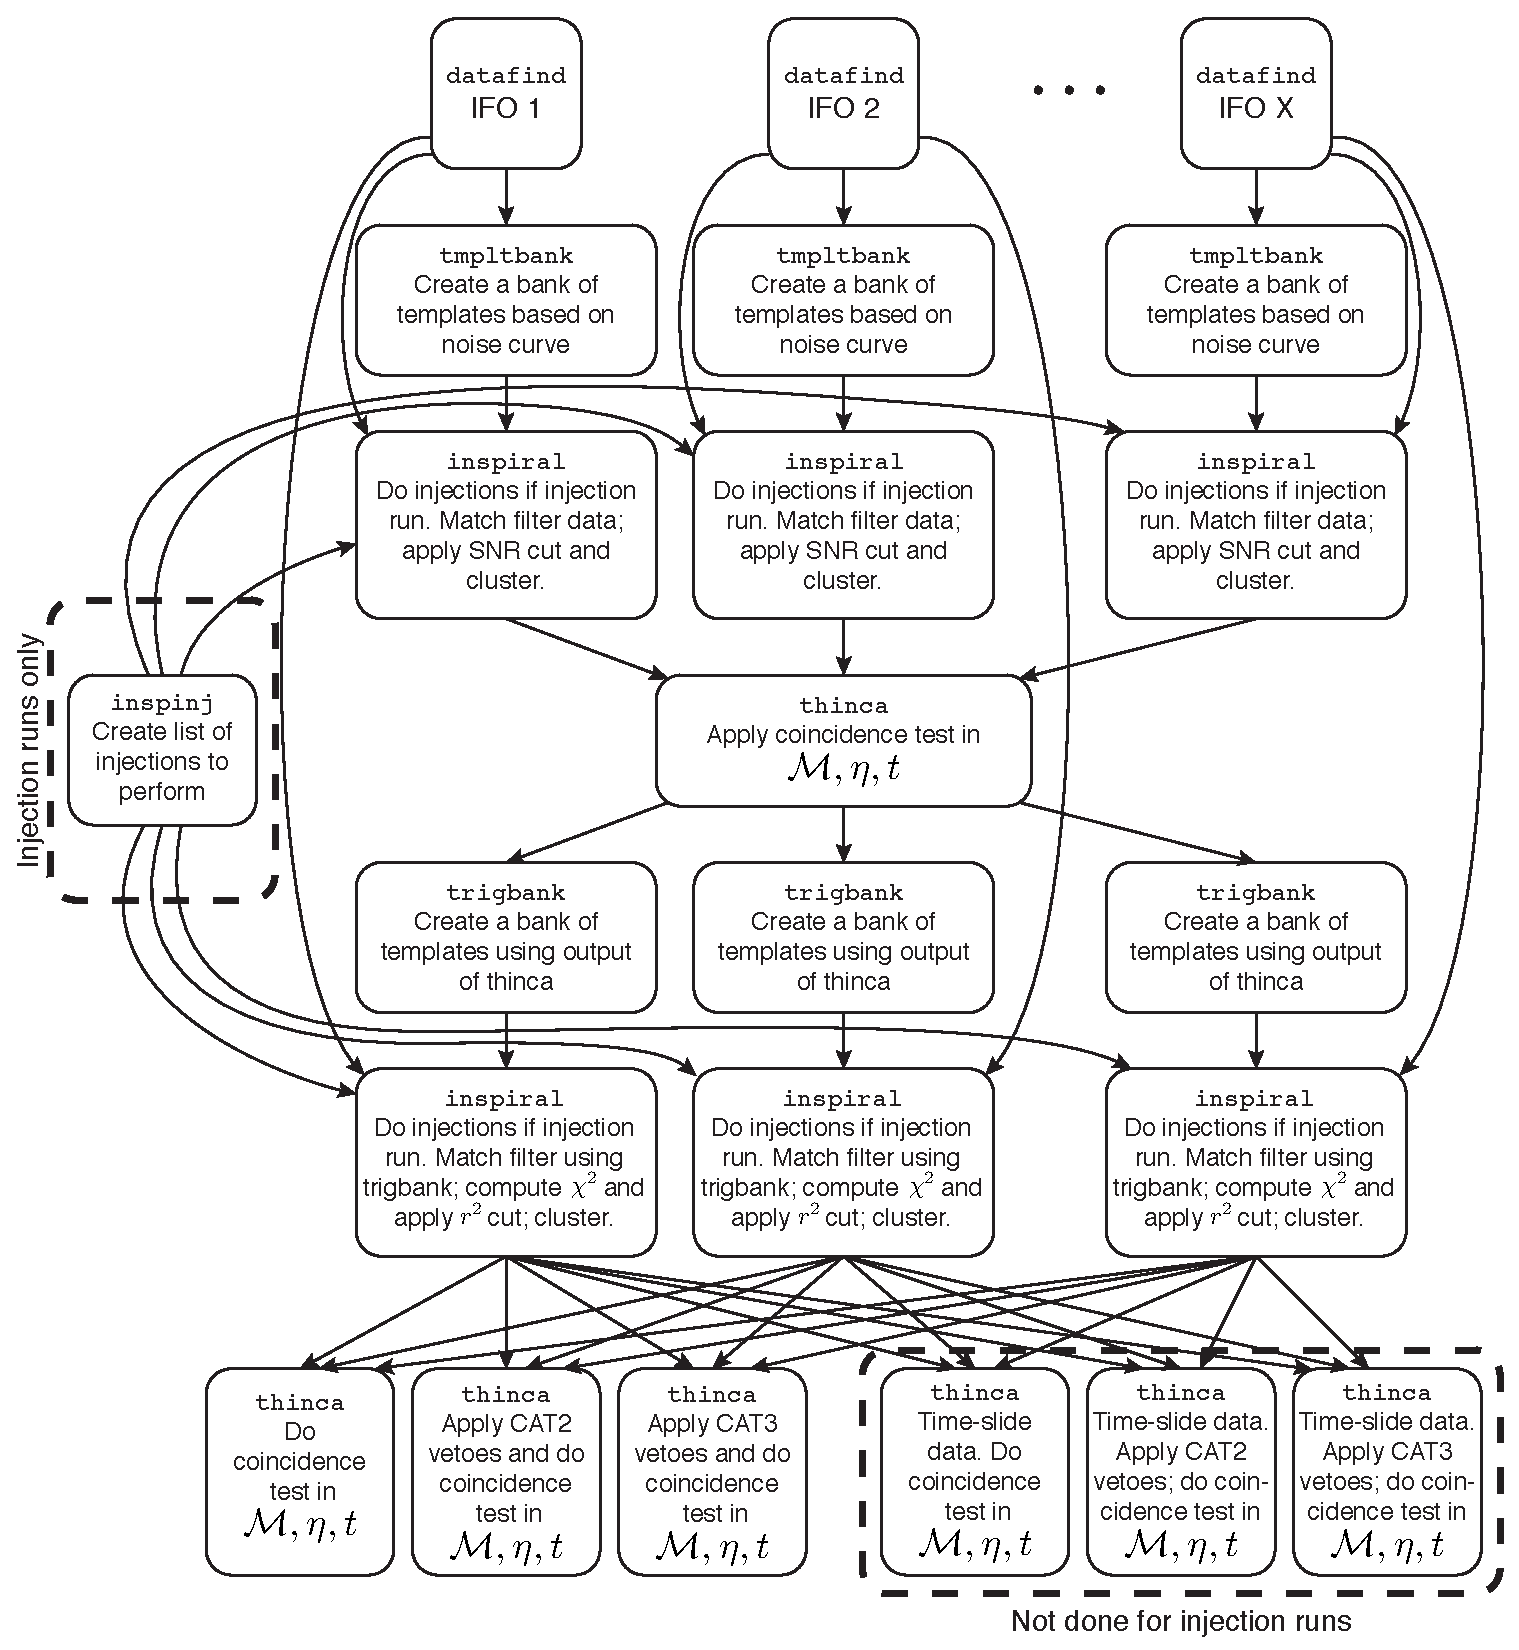
\includegraphics[width=\linewidth]{figures/detchar/HIPEDiagram}
  \caption[Structure of the full iHope search]{
  \label{f:hipe}
Structure of the full iHope search.  For details see (\Note{Collin's
thesis}).
}
\end{figure}%

%do analysis
%record science triggers
%cluster 30 ms     determine cat 1
%cluster 16 sec    determine cat 1 + cat 2
%                  ...

%filter and record

\section{The Daily Ihope report pages}

Much of the utility of the daily runs was in the use of the resulting
triggers to identify data quality issues and quantify the value of
proposed vetoes.  Some of these uses will be discussed in
section~\ref{sec:applications_vetoes}.  In addition to the triggers
the daily pipeline also produced a large number of plots and reports,
organized into web pages that were available to the collaboration.
Data analysts could use these pages to spot potential problems for the
full analysis and begin more detailed followup studies.  

We now summarize the contents of the daily pages. Each report and plot
is made for each combination of the following:

\begin{itemize}
\item IFO: H1, L1 and V1
\item Cluster level: Unclustered, 30 ms clustering, 16 second
clustering
\item Veto level: Show all triggers in science time (level ``0''),
only those not removed by category 1 vetos, only those not
removed by categories 1 or 2, or only those note removed by
categories 1,2 and 4.  Hardware injections vetos (category 3) were not 
applied so that we could determine whether category 4 vetoes were 
remove them.
\end{itemize}

Each of these features could be set independently.  The top-level web
interface for a sample day is shown in figure~\ref{f:daily_ihope_top}.

\begin{figure}
  \includegraphics[width=\linewidth]{figures/detchar/daily_ihope_top}
  \caption[Top-level web interface for daily ihope]{
  \label{f:daily_ihope_top}
Top-level web interface for daily ihope.  Options can be selected with
the controls on the left hand side, when a button is clicked the
contents region is immediately replaced.  The default view is the one
shown here; the analysis time and veto efficiency at cat 1 for the
Hanford detector.}
\end{figure}%

The available reports can bee seen at the bottom of the list of
controls in figure~\ref{f:daily_ihope_top}:

\weakheader{1. Analysis time and veto usage.}

This report shows the total time analyzed, the vetoes applied beyond
those applied at the previous level, the \emph{efficiency} (percentage
of triggers removed) and \emph{deadtime} (percentage of time removed)
by each veto.  In addition the ratio of efficiency over deadtime is
reported as a measure of quality of the veto.  A random veto would
result in an efficiency-over-deadtime of approximately 1, a
finely-tuned veto that removes short, loud events that ring off the
entire template bank would have a much higher ratio.   An example is
shown in figure~\ref{f:daily_ihope_vetousage}.


\begin{figure}
  \includegraphics[width=\linewidth]{figures/detchar/vetousage.png}
  \caption[Sample veto usage report from Aug 19, 2010]{
  \label{f:daily_ihope_vetousage}
A sample veto usage report, see text for explanation.  Note that 62.66\% of
all triggers were contained in 14.51\% of time, and the DMT flagged this time
with elevated seismic activity from 3-10 Hz at the LVEA.}
\end{figure}%

\weakheader{2. Loudest triggers}

This report was only run for 16-second-clustered triggers.  Loud
glitches tend to produce families of triggers, without clustering the
loudest triggers from each day would likely result from one underlying
event.  This report considers two classes of triggers; those where no
data quality flag was active and those where at least one flag was
active.  A sample report is shown in
figure~\ref{f:daily_ihope_loudest}.  For the five triggers with
highest new SNR in each category a summary was presented along with a
link to an \emph{omega scan}.  The omega pipeline is described in
(\checkme{omega refs}).  Omega scans are a kind of time-frequency
plot.  They are especially useful as they may be run on all auxiliary
channels recorded by the instruments and therefore provide a visual
aid to detecting coupling between auxiliary channels and the
gravitational wave readout channel.  These can be used to suggest
mechanisms behind glitches, especially those that were not already
marked by a DQ flag.  In addition, over time repeated shapes in the
omega scan can pinpoint underlying problems in the instruments that
need to be addressed.  A few images from one of the glitches in
figure~\ref{f:daily_ihope_loudest} is shown in
figure~\ref{f:daily_ihope_loudest_omega}.

\begin{figure}
  \includegraphics[width=\linewidth]{figures/detchar/loudest.png}
  \caption[Sample loudest trigger report from Aug 19, 2010]{
  \label{f:daily_ihope_loudest}
A sample report on loudest triggers, see text for explanation.  Note the
rightmost column is populated by
the \texttt{ligolw\_dq\_query} program in the \texttt{--report} mode.}
\end{figure}%



\begin{figure}
  \includegraphics[width=0.5\linewidth]{figures/detchar/966222827_940673828_H1_LSC-DARM_ERR_1_00_spectrogram_whitened.png}
  \includegraphics[width=0.5\linewidth]{figures/detchar/966222827_940673828_H0_PEM-ISCT1_ACCX_1_00_spectrogram_whitened.png}
  \caption[Omega scans from the loudest H1 trigger in figure \ref{f:daily_ihope_loudest}]{
  \label{f:daily_ihope_loudest_omega}
Omega scans from the loudest H1 trigger in figure
\ref{f:daily_ihope_loudest}.
Note the trigger closely follows a loud
event in one of the accelerometers on an instrument table.}
\end{figure}%


\weakheader{3. Hardware injections}

This report was generated by code written by John Veitch  at Cardiff
University.  It compared the list of injections, published as an XML
file available from a web site, with the list of analysis times and
triggers.  The results were plotted to indicate whether each injection
was found, missed, or not analyzed.


\weakheader{4. SNR histograms}

These plots show the number of triggers as a function of SNR and new
SNR.  As noted in section \ref{sec:ihope_match_filter}, in Gaussian
noise the number of triggers should be proportional to
$\exp(-\rho^2/2)$.  These plots therefore show the degree of
``non-Gausianity'' in the data.  A common use for these plots was to
flip between veto levels to get a sense of how well the cumulative
vetoes were cleaning the data, as shown in figure
\ref{f:daily_ihope_gaussianity}.

Similarly figure~\ref{f:daily_ihope_gaussianity_newsnr} shows histograms
of the triggers in new SNR.  The total number of triggers is greatly
reduced because many high-SNR triggers have $\newsnr < 5$ , where the
plot cuts off.  While triggers with such low $\newsnr$ values are not
excluded from later stages of analysis in the full pipeline, it is
extremely unlikely that the resulting combined new SNR will be high
enough to stand above background.

In addition to the lower number of triggers overall, the new SNR plot
is closer to a straight line indicating behavior closer to that
expected in Gaussian noise.  However, detchar improves the situation
still further, as the number of triggers is reduced at veto category
4.

However, there is one trigger with $\newsnr = 8$ that is not removed
by any veto.  Such an outlier warrants further investigation, which
here is provided by the loudest events page an example of which is
shown in~\ref{f:daily_ihope_loudest}.  The omega scan from the time of
this event is shown in figure~\ref{f:daily_loudest_glitch}, and it
clearly rules out a gravitational wave as the source of this trigger.
This illustrates the important point that new SNR can be fooled, and
hence continued human participation in detchar is necessary.

\begin{figure}
  \includegraphics[width=0.5\linewidth]{figures/detchar/H1_1_UNCLUSTERED_snr_hist.png}
  \includegraphics[width=0.5\linewidth]{figures/detchar/H1_4_UNCLUSTERED_snr_hist.png}
  \caption[Trigger SNR histograms for H1]{
  \label{f:daily_ihope_gaussianity}
Sample trigger histograms by SNR.  The dashed line shows the
expected values in Gaussian noise.  The dot indicates the cumulative
number of triggers with new SNR greater than 200.  Note that at veto
category 4 (right) the histogram is closer to the expected line than
it is at category 1 (left).  This indicates the degree to which data
quality has removed non-Guassian noise.}
\end{figure}%



\begin{figure}
  \includegraphics[width=0.5\linewidth]{figures/detchar/H1_1_UNCLUSTERED_new_snr_hist.png}
  \includegraphics[width=0.5\linewidth]{figures/detchar/H1_4_UNCLUSTERED_new_snr_hist.png}
  \caption[Trigger new SNR histograms for H1]{
  \label{f:daily_ihope_gaussianity_newsnr}
Sample trigger histograms by new SNR. The data is much cleaner than
the SNR histograms, but there is still an outlier at $\newsnr=8$.}
\end{figure}%



\begin{figure}
  \includegraphics[width=\linewidth]{figures/detchar/966281824_963867187_H1_LSC-DARM_ERR_1_00_spectrogram_whitened}
  \caption[Omega scan of the loudest new SNR trigger]{
  \label{f:daily_loudest_glitch}
The omega scan from the outlier with new SNR=8 that survives all
automated data quality vetoes.  Many auxiliary channels showed the
same behavior at this time.  This is clearly not a gravitational wave,
but was not removed by either signal-based vetoes or data quality
vetoes.}
\end{figure}%


\weakheader{5. The ``glitchgram''}

This was an ``at-a-glance'' summary of the day, showing every trigger
color-coded by SNR.  This highlighted times of loud triggers as well
as dense regions indicating ``grumbly'' times.  A sample is shown in
figure \ref{f:daily_ihope_glitchgram}.

\begin{figure}
  \includegraphics[width=\linewidth]{figures/detchar/H1_1_UNCLUSTERED_glitchgram.png}
  \caption[The Aug 19th daily ihope ``glitchgram'']{
  \label{f:daily_ihope_glitchgram}
A sample ``glitchgram.'' Blue dots have
new snr values below 8, green have values between 8 and 16,
and red have values above 16.  Template length was chosen as the Y
axis in order to capture a feature of the templates that is not
specific to gravitational wave signals, such as chirp mass.
Note the break at 4.3 seconds, corresponding to the
chirp mass at which the bank switches from an overlap of 0.95 to 0.5.
Comparing to figures 3 and 4 shows the same 
excess of triggers after 12:00.  No data is analyzed after 21:00
because ihope requires at least 2048 contiguous seconds to estimate
the PSD and all data after this time was in smaller segments.}
\end{figure}%


\weakheader{6. Rate vs. Time and SNR vs. Time}

These plots complimented the glitchgram by breaking the triggers up
differently.  The rate plot (figure~\ref{f:daily_ihope_rate_v_time})
showed average number of triggers over 1-minute intervals.  The SNR
plot (figure~\ref{f:daily_ihope_snr_v_time}) showed the SNR of every
trigger as a function of time.  These tend to be correlated, as loud
glitches ring off the entire bank and produce large numbers of
triggers.  The plots were accompanied by tables showing the times
where the rate of triggers exceeded 500 Hz for more than one second,
and exceeded 200 Hz for more than 10 seconds.

\begin{figure}
  \includegraphics[width=\linewidth]{figures/detchar/H1_0_UNCLUSTERED_rate_vs_time.png}
  \caption[Daily ihope rate plot]{
  \label{f:daily_ihope_rate_v_time}
Sample rate plot, showing rate in Hz (averaged over
1-minute intervals) as a function of time.  Note that the rates
increase after 12:00.  This was due to increased seismic noise.}
\end{figure}%

\begin{figure}
  \includegraphics[width=\linewidth]{figures/detchar/H1_0_UNCLUSTERED_snr_vs_time.png}
  \caption[Daily ihope SNR plot as a function of time]{
  \label{f:daily_ihope_snr_v_time}
Sample plot of SNR as a function of time.  The density of
triggers increases somewhat after 12:00 and there are more loud
outliers.  However the change in behavior is better seen in 
figure \ref{f:daily_ihope_rate_v_time}.}
\end{figure}%


\weakheader{7. Breakdown by template}

This page showed several histograms of number of triggers as a
function of the length of templates in seconds.  Examples of the
standard histograms are shown in
figure~\ref{f:daily_ihope_trig_histograms}, they show that most of the
triggers come from short templates, and templates shorter than 5
seconds produce up to six times as many triggers as shorter templates.

Figure~\ref{f:count_per_template} shows the same information as a map
of the template bank, color-coded to indicate how many triggers each
template produced.  Figure~\ref{f:daily_ihope_time_mass} breaks this
same information up by time and template mass.

Qualitatively these plots do not change much day-by-day, and so these
plots were not often used.  However, they did prompt a change to
the analysis made early in the S6 run, see
section~\ref{sec:applications_pipeline}.

\begin{figure}
  \includegraphics[width=0.5\linewidth]{figures/detchar/H1_1_UNCLUSTERED_mass_hist}
  \includegraphics[width=0.5\linewidth]{figures/detchar/H1_1_UNCLUSTERED_mass_hist_norm}
  \caption[Histograms of trigger rates by template length]{
  \label{f:daily_ihope_trig_histograms}
Histograms of trigger rates by template length in daily ihope.  The
plot on the left combines all templates, the plot on the right
normalizes by plotting (number of triggers resulting from templates of
length $x$) divided by (number of templates of length $x$).
}
\end{figure}%

\begin{figure}
  \includegraphics[width=\linewidth]{figures/detchar/H1_1_UNCLUSTERED_template_counts}
  \caption[Triggers per template]{
  \label{f:count_per_template}
The daily template bank, color-coded to show how many triggers each
template produced.  Note that the template in the upper-right corner,
which is the template of shortest duration, produced approximately 1.3
times as many triggers as the next most active.
}
\end{figure}%


\begin{figure}
  \includegraphics[width=\linewidth]{figures/detchar/H1_1_UNCLUSTERED_hexmass}
  \caption[Trigger rates as a function of time and template length]{
  \label{f:daily_ihope_time_mass}
Trigger rates as a function of time and template length.  The elevated
trigger rate after 12:00 is visible here as well.  Note that
particularly loud glitches, such as that around 19:30, ring off the
entire bank.
}
\end{figure}%


\weakheader{8.  The $\chisq$ test}

These plots showed all triggers with SNR values on the $x$-axis and
$\chisq / (2p-2)$ (the reduced $\chisq$) on the $y$-axis as a way to
visualize the glitchiness of the data.  These plots are most useful
when compared to a reference plot generated from a day of simulated
Gaussian noise, shown in figure \ref{f:gaussian_snr_chisq}, and
comparing the plots at different veto levels, shown in figure
\ref{f:daily_ihope_snr_chisq}.

\begin{figure}
\includegraphics[width=0.85\linewidth]{figures/detchar/GAUSSIAN_0_UNCLUSTERED_chisq.png}
\caption[SNR/reduced $\chisq$ values in Gaussian noise]{
\label{f:gaussian_snr_chisq}
The SNR/reduced $\chisq$ plane for a reference day of
Gaussian noise.  This is the product of a $\chisq$ distribution on the
$y$ axis and a Gaussian distribution on the $x$ axis.}
\end{figure}%

\begin{figure}
  \includegraphics[width=0.5\linewidth]{figures/detchar/H1_0_UNCLUSTERED_chisq.png}
  \includegraphics[width=0.5\linewidth]{figures/detchar/H1_4_UNCLUSTERED_chisq.png}
  \caption[SNR/reduced $\chisq$ plots of H1 data.]{
  \label{f:daily_ihope_snr_chisq}
SNR/reduced $\chisq$ plots of H1 data.  The expected shape
of figure \ref{f:gaussian_snr_chisq} is discernible, but there are
long tails of non-Gaussian glitches.  The sharp cutoffs arise 
from thresholds within the inspiral code, see section
\ref{sec:analysis_trigger_selection}.  There is a further
population extending to the upper right at category 0 (left) that is
removed by vetoes in category 4 (right).}
\end{figure}%


\section{Applications of daily ihope to pipeline tuning}
\label{sec:applications_pipeline}

Early in S6 there were frequent instances where the full analysis ran
into difficulty.  This was characterized by individual programs taking
abnormally long to complete, consuming far more than the expected
amount of memory, or failing outright.  The problematic jobs tended to
be individual runs of the \texttt{trigbank} program (see
figure~\ref{f:hipe}); this is the step where triggers from the first
stage are examined to determine which templates need to be used at the
second stage (see figure~\ref{f:hipe}).  Comparing the times that
caused problems to the daily pages immediately revealed a correlation
-- times over which \texttt{trigbank} were unable to run were those
where the rates of triggers were abnormally high.

In S5 and the early weeks of S6 triggers were clustered using a method
called \emph{trigscan}~\cite{SenguptaTrigScan:2008} which attempts to
collapse clusters of triggers that are close in time and parameters to
a single most-significant trigger.  Early versions of the daily page
did this clustering as well, and comparison between the unclustered
and trigscan-clustered triggers revealed that even after clustering
periods of high trigger rates remained~\footnote{Trigscan worked well
in S5, it is not known why it did not work as well in S6.  It is
possible that the instruments were simply more glitchy in the early
days of S6.  However, in order to group triggers together trigscan
must use the bank metric, which was correct in S5 when 2.0 pN
templates were used but incorrect in S6 when the analysis moved to 3.5
pN templates (see section~\ref{sec:bank_metric}).  Some preliminary
investigations were performed, but results were inconclusive}.  This
is illustrated in figure~\ref{f:daily_ihope_high_rates}.  There is a
short period of high trigger rate around 05:40 which remained high
after clustering.  A run of \texttt{trigbank} processing this time was
unable to complete.

The possibility of vetoing such glitchy periods was raised, and this
could have been easy to accomplished using the rate information from
daily ihope.  However, such vetoes would have needed to be category 1 to
avoid the problem, which would mean subdividing science segments and
possibly losing short segments.  Instead we replaced trigscan with
fixed 30-millisecond clustering windows, after studies of found/missed
injections determined that this change did not harm the search
efficiency. 

\begin{figure}
  \includegraphics[width=0.5\linewidth]{figures/detchar/20090806_H1_0_UNCLUSTERED_rate_vs_time}
  \includegraphics[width=0.5\linewidth]{figures/detchar/20090806_H1_0_TS_CLUSTERED_rate_vs_time}
  \caption[Problematic times identified by daily ihope]{
  \label{f:daily_ihope_high_rates}
Problematic times identified by daily ihope.  The plot on the left
shows the rate of triggers over the day without any clustering.  Note
the sudden jump in rate at 5:40.  On the right, the same plot after
clustering triggers with the trigscan algorithm.  The overall rate has
been reduced by about a factor of two, indicated by the different
scales on the y axes.  However, the rate remains high enough to cause
problems.
}
\end{figure}%

At the start of S6 the range of the low-mass search extended up to $35
\msun$, as it did in S5.  However, along with times of high trigger
rates, the daily ihope pages indicated that most of the triggers were
coming from the high-mass end of the bank.  This behavior is expected,
as it is easier for short templates to match against glitches, but the
trigger histograms highlighted the extent to which this was a problem.
A sample plot of triggers per template from early S6 is shown on the
left of figure~\ref{f:daily_ihope_el_glitcho}.  It shows that the
shortest template in the bank, with $m_1 = m_2 = 17.5 \msun$ was
producing significantly more triggers than any other template.  In
part this was due to a bug in the template bank code, that caused this
template to appear twice in some banks.  In part the abundance of
triggers from this template is due to it appearing in every bank
throughout the day, whereas other templates tend to get repositioned
as the noise curve changes.  Even taking these effects into account,
most of the triggers come from templates shorter than 5 seconds, as
seen on the right of figure~\ref{f:daily_ihope_el_glitcho}.

The fixed clustering window means that only the loudest trigger in a
30-millisecond window will be passed to subsequent stages of the
analysis.  Given the numbers of triggers from short templates there
was concern that a loud, short glitch could mask a quieter trigger
from a binary neutron star coalescence.  We therefore decided to limit
the low-mass search to $M < 25 \msun$ after comparing found/missed
plots of injections in the same weeks with the different mass ranges,
and determining that the smaller bank did as well or better than the
larger bank.


\begin{figure}
  \includegraphics[width=0.5\linewidth]{figures/detchar/20090806_H1_0_UNCLUSTERED_template_counts}
  \includegraphics[width=0.5\linewidth]{figures/detchar/20090806_H1_0_UNCLUSTERED_mass_hist_norm}
  \caption[Problematic templates seen in daily ihope]{
  \label{f:daily_ihope_el_glitcho}
Problematic templates seen in daily ihope.  This shows the equivalent
of figures~\ref{f:daily_ihope_time_mass} and
\ref{f:count_per_template} from an earlier version of daily ihope and
an earlier version of the CBC search.  Note the excess of triggers
from the high-mass end of the bank, corresponding to shorter
templates.
}
\end{figure}%



\section{Applications of daily ihope to individual vetoes}
\label{sec:applications_vetoes}

In addition to tracking the performance of the pipeline as a whole,
daily ihope was used to flag numerous glitch mechanisms throughout the
course of S6.  Such glitches typically showed up in the rate vs. time
plot, the SNR vs. time plot, and/or the list of loudest triggers.
Often these were spotted either by individuals reviewing the pages on
a daily basis, by an individual in the CBC group assigned  to do
glitch studies preceding a run of the full analysis pipeline, or by
the group during reviews of these studies.

As patterns emerged from these results members of the detector
characterization group would work with the commissioners to identify
the underlying causes, and simultaneously work with data analysts to
develop and test vetoes.  Often these vetoes were verified by running
a script, \texttt{lalapps\_check\_flag} which, given a file
containing veto segments and a time range would report on the
efficiency and deadtime of the veto by applying it to the daily ihope
triggers over the specified time range.  The file could be generated
from an existing flag in the database using {\texttt
ligolw\_dq\_query} (see chapter~\ref{ch:segdb}), or it could be
generated by a script looking at auxiliary channel information
provided by Omega or klinewelle triggers.

We now give examples of the use of daily ihope in constructing vetoes
at each level.

\subsection{Category 1}

\weakheader{Glitches from the Thermal Compensation System}

The design of the LIGO mirrors accounted for the fact that in
operation they would be heated by the laser and the radius of
curvature would change.  However, in S6 as we moved to higher laser
power the mirror's absorption of energy was larger than expected and
the mirror overheated and deformed more than expected~\cite{}.  To
correct for this a compensating laser was added that would heat the
mirror in a ring in order to restore the radius of curvature to an
optimal value.  However, this laser would occasionally glitch, kicking
the mirror and producing loud noise in the detector.

The identification of these glitches was straightforward; they were
often the loudest glitches of the day and were readily visible in the
daily ihope ``loudest trigger'' report, as well as similar reports
generated by KW and Omega.  The cause was similarly easy to identify,
as the omega scans generated by daily ihope showed egregious behavior
in the TCS channels.  An automated veto based on a threshold value in
the TCS channel was added to the DMT at category 2.  However, some
instances were loud enough to interfere with the CBC pipeline in
surrounding times, hence it was decided to veto these times at
category 1.  These features are illustrated in
figure~\ref{f:daily_ihope_tcs}.  


%
% P. Willems, "Thermal Compensation in the LIGO Gravitational-Wave
% Interferometers," in Adaptive Optics: Methods, Analysis and
% Applications, OSA Technical Digest (CD) (Optical Society of America,
% 2009), paper AOThA5.
% http://www.opticsinfobase.org/abstract.cfm?URI=AO-2009-AOThA5
% 

\begin{figure}
  \includegraphics[width=0.5\linewidth]{figures/detchar/20100217_H1_0_UNCLUSTERED_snr_vs_time} 
  \includegraphics[width=0.5\linewidth]{figures/detchar/20100217_H1_0_UNCLUSTERED_rate_vs_time} \\
  \includegraphics[width=0.5\linewidth]{figures/detchar/950432156_482177734_H1_LSC-DARM_ERR_4_00_spectrogram_whitened}
  \includegraphics[width=0.5\linewidth]{figures/detchar/950432156_482177734_H1_TCS-ITMY_PD_ISS_OUT_AC_4_00_spectrogram_whitened}
  \caption[TCS glitch in daily ihope and omega]{
  \label{f:daily_ihope_tcs}
TCS glitches in daily ihope and followup omega scans.  The top left
shows the SNR as a function of time, the loudest triggers are all TCS
glitches.  Note that each loud glitch comes in the form of a ``tower''
containing many triggers.  This phenomena will be discussed further in
section~\ref{ssec:penguins}.  This is further illustrated by the trigger
rate plot (top right), which shows elevated trigger rates at the times
of the glitch.  Note that around the time of the glitch the trigger
rate actually {\it drops} significantly.  This will be discussed in
section~\ref{ssec:sarlacc}, but indicates that the glitches are loud
enough to interfere with the analysis in surrounding times, justifying
the use of a CAT 1 veto.  The lower left plot shows the omega scan
of the gravitational-wave output channel at the time of the loudest
glitch, clearly showing that this is not a gravitational wave.  The
lower right plot shows the omega scan of a channel monitoring the TCS,
identifying it as the source of the glitch.}
\end{figure}%


\weakheader{Grid glitches}

This was a loud, broad-band glitch that produced a grid of triggers in
the KW pipeline's time-frequency plane, where the phenomena was first
seen.  They also showed up in the daily ihope rate and SNR plots as
loud triggers accompanied by elevated trigger rates, as shown in
figure~\ref{f:omega_grid}.  These also often appeared on the
daily list of loudest glitches, the omega scans generated by daily
ihope showed problems in magnetometers and the output mode cleaner
photodiodes, this is shown in figure~\ref{f:omega_grid}.  As with the
TCS glitches, instances that showed up particularly loudly in daily
ihope were hand-vetoed at category 1.  The problem was eventually
traced to a power supply, once this was resoldered the problem
disappeared.

% https://wiki.ligo.org/foswiki/bin/view/DetChar/CurrentUnvetoedGlitchClasses
% https://wiki.ligo.org/DetChar/H1GridGlitchStory

% Example: 
% tconvert 963852915
% Jul 22 2010 16:55:00 UTC

\begin{figure}
  \includegraphics[width=0.5\linewidth]{figures/detchar/20100722_H1_0_UNCLUSTERED_newsnr_vs_time}
  \includegraphics[width=0.5\linewidth]{figures/detchar/20100722_H1_0_UNCLUSTERED_rate_vs_time}
  \caption[Grid glitches in daily ihope] {
  \label{f:daily_ihope_grid}
Grid glitches as seen by daily ihope.  The plot on the left shows
$\newsnr$, with the grid glitches indicated by arrows pointing above
the range at which the plot cuts off (auto-scaling of this plot was
removed from daily ihope to prevent a single loud glitch from
squeezing all the other data to a thin region at the bottom of the
plot).  Note that the high value indicates that this glitch is fooling 
the $\chisq$ signal-based veto.  The plot on the right shows the
associated increase in trigger rate.
}
\end{figure}%

\begin{figure}
  \includegraphics[width=\linewidth]{figures/detchar/963853263_154296875_H1_LSC-DARM_ERR_1_00_spectrogram_whitened}
  \includegraphics[width=0.5\linewidth]{figures/detchar/963853263_154296875_H0_PEM-BSC1_MAG1X_1_00_spectrogram_whitened}
  \includegraphics[width=0.5\linewidth]{figures/detchar/963853263_154296875_H1_OMC-QPD3_SUM_IN1_DAQ_1_00_spectrogram_whitened}
  \caption[Grid glitches in omega]{
  \label{f:omega_grid}
Omega scans of the grid glitch flagged as the loudest trigger of the
day and visible as an arrow in figure~\ref{f:daily_ihope_grid}.  At
the top, the gravitational-wave output channel, and at the bottom two
channels that were associated with this class of glitch.
}
\end{figure}%


\subsection{Category 2}

\weakheader{The spike glitch}

The spike glitch was a very loud, very short ``bang'' in the
Livingston detector, characterized by a sudden drop in \darmerr
immediately followed by a sharp increase.  An example is shown in
figure~\ref{f:spike_glitch_example}.  In some cases there were a few
cycles of ringing before the channel settled back down.  These often
produced SNR values of several thousand.  The $\chisq$ values were
typically large for the events themselves, resulting in negligible
$\newsnr$ values.  However, the triggers in the tails (see
section~\ref{ssec:penguins}) could have large new SNR values.  A
sample daily ihope plot with several spike glitches and representative
omega scans are shown in figure~\ref{f:daily_spikes}.

\begin{figure}
  \includegraphics[width=\linewidth]{figures/detchar/spike_glitch_example}
  \caption[The spike glitch]{
  \label{f:spike_glitch_example}
A sample spike glitches in \darmerr.  Note the characteristic
down-up-down pattern, and short timespan.}
\end{figure}%

Despite a great deal of effort by lots of people, the cause of these
glitches was never identified.  However, the distinctive shape allowed
the creation of an automated veto.  \texttt{LSC\_STRAIN} was sampled
every half-millisecond, giving a time series $x_i$.  For each sample
$i$ the quantity 

\begin{equation*}
x_i - 2 x_{i+1} + x_{i+2} 
\end{equation*}

was calculated, values exceeding a threshold indicated a possible
spike and the time was flagged in the segment database.  Not every
time so-flagged was a spike, but every instance indicated a
potentially problematic rapid fluctuation in the data.



% https://wiki.ligo.org/foswiki/bin/view/DetChar/S6L1OMCGlitchVeto

% DCH-SPIKE_GLITCH (0,4)

% Example 947204646.611816406
% Jan 11 2010 00:23:51.611816406 UTC == SNR 8849


\begin{figure}
  \includegraphics[width=\linewidth]{figures/detchar/20100111_L1_0_UNCLUSTERED_snr_vs_time} \\
  \includegraphics[width=0.5\linewidth]{figures/detchar/947204646_611816406_L1_LSC-DARM_ERR_1_00_spectrogram_whitened}
  \includegraphics[width=0.5\linewidth]{figures/detchar/947204646_611816406_L1_LSC-DARM_ERR_1_00_timeseries_raw}
  \caption[Spike glitch in daily ihope and omega]{
  \label{f:daily_spikes}
  Spike glitches in daily ihope and a typical omega scan.  At the top
a daily ihope SNR-vs-time plot, showing several spike glitches with
SNRs of several thousand.  On the bottom, the loudest of these spike
glitches in an omega scan, showing the time-frequency plot (left) and
unfiltered time series (right).  The sharp drop-rise-drop of the time
series behavior was reasonable well-captured by the filtered used to
create data quality segments.
}
\end{figure}%

\weakheader{HEPI glitches}

Livingston is subject to seismic activity, both natural and
anthropogenic, that does not effect the Hanford detector.  In order
for the L1 detector to achieve the same low-frequency response it is
therefore necessary to take additional steps.  The Hydraulic External
Pre-Isolation (\emph{HEPI}) system sits between the ground and
chambers containing optical components and provides a layer of active
seismic isolation.  This can reduce noise in the 1-3 Hz band by a few
percent~\cite{Wen:thesis}.

In early 2010 it was noticed that the daily ihope triggers contained
several instances with SNRs above 600 even after applying all known
vetoes through category 4.  This included removal of spike glitches
and application of the use-percentage vetoes (discussed in the next
section).  Followup of these triggers in the daily loudest-glitch
reports showed that they were all accompanied by loud glitches in the
HEPI channels.  Samples are shown in figure~\ref{f:daily_hepi}.

A trial veto was created by scanning the auxiliary channel time series
for values exceeding 25,000.  This veto was tested by applying it to
the remaining daily ihope triggers, and it was found to be very
effective.  Histograms of triggers before and after application of
this veto are shown in figure~\ref{f:hepi_veto_effectiveness}.  After
this confirmation the veto was applied at category 2 to the full
search.

A great deal of work was done on HEPI during this period, and after
Jan 10, 2010 the problem ceased.

% DCH-SEI_ITMY_Y_OVER_25000
% example 946834715.499755859 == Jan 06 2010 17:38:20 UTC
% https://ldas-jobs.ligo.caltech.edu/~cbc/ihope_daily/201001/20100106/
% 5th loudest in day
%
% https://wiki.ligo.org/foswiki/bin/view/DetChar/CBC_S6B_L1_SingleDetectorLoudest
% After applying CAT 2, 3, and 4, including UPV and the Spike glitch
% veto, there are still many loud triggers in the CBC single-detector
% background. This does not include the effect of chi squared or
% coincidence. The triggers above SNR 600 are: 
%
% https://ldas-jobs.ligo.caltech.edu/~lundgren/DataQuality/Issues/HEPI/L1-S6B2-snrhist_Cat1234_Spike_HEPI.png
%
% http://www.ligo.caltech.edu/LIGO_web/0409news/0409liv.html


\begin{figure}
  \includegraphics[width=0.5\linewidth]{figures/detchar/20100106_L1_0_UNCLUSTERED_snr_vs_time}
  \includegraphics[width=0.5\linewidth]{figures/detchar/946834715_499755859_L1_LSC-DARM_ERR_1_00_spectrogram_whitened} \\
  \includegraphics[width=0.5\linewidth]{figures/detchar/946834715_499755859_L1_SEI-ITMY_Y_1_00_timeseries_raw}
  \includegraphics[width=0.5\linewidth]{figures/detchar/946834715_499755859_L1_SEI-ITMY_Y_1_00_spectrogram_whitened}
  \caption[The HEPI glitch in daily ihope and Omega]{
  \label{f:daily_hepi}
The HEPI glitch in daily ihope and Omega.  On the top left, the SNR
values for the day including a HEPI glitch at 17:38, as identified by
the ``loudest glitches'' report.  On the top right, this event in
\darmerr.  On the bottom left the time-frequency plot of a HEPI
auxiliary channel, and on the bottom right the unfiltered time series
of this same channel, showing that it has exceeded the threshold of
25,000}
\end{figure}%

\begin{figure}
  \includegraphics[width=\linewidth]{figures/detchar/L1-S6B2-snrhist_Cat1234_Spike_HEPI}
  \caption[Effectiveness of the HEPI veto] {
  \label{f:hepi_veto_effectiveness}
Effectiveness of the HEPI veto. The green line shows the number of
daily triggers after applying all known vetoes, including the removal
of spike glitches.  The blue line show counts after the additional
HEPI veto is applied.  Note that the highest SNR is reduced from 
4,000 to 600, along with a reduction of triggers at SNRs down to 
$~ 10$.}
\end{figure}


\subsection{Category 4}

% https://wiki.ligo.org/foswiki/bin/view/DetChar/H1LVEASEISZS6Cflag

\weakheader{Automated vetoes}

There were three uses of the daily triggers through S6.  The first
two, the daily pages and ad-hoc veto studies, have already been
discussed.  The third was as input to systematic automated veto
studies.

\emph{SeisVeto}~\cite{} compared low-frequency triggers from Omega
running on seismic PEM channels to daily ihope triggers using the
\emph{HVeto}~\cite{} algorithm.  Times of high correlation were
flagged with category 4 vetoes, which could achieve up to 62\%
efficiency with only 6\% deadtime.

The \emph{Used Percentage Veto} (UPV) program looked for correlations
between triggers from \darmerr and auxiliary channels using a figure
of merit defined as

\begin{equation*}
\textrm{Used Percentage}(\rho) \equiv 100 \times
N_\textrm{coinc}(\rho) / N_\textrm{total}(\rho)
\end{equation*}

where $N_\textrm{total}(\rho)$ is the total number of triggers from
the auxiliary channel above significance threshold $\rho$ in the
analysis time, and $N_\textrm{coinc}(\rho)$ is the number of trigger
from the auxiliary channel that lie within a second of a trigger from
\darmerr.  Intervals where this percentage exceeded 50\% were entered
into the segment database and applied as category 4 vetoes.  Although
UPV was originally developed using KW triggers for both \darmerr and
auxiliary channels, it was modified during S6 to accept triggers from
daily ihope.  The resulting analysis was rerun weekly.


% UPV-IHOPE_H1_ASC_WFS2_IY_8_256_100 (in C) and more
% (tconvert 957191412, May 06 2010 14:29:57 UTC)
% Accompanied by rate > 500 Hz (=866) for 4 seconds, slight elevation in SNR

An example is shown in figure~\ref{f:daily_upv}.  During the week
including this day UPV determined that the instrumental channel
\texttt{ASC-WFS2\_IY} \Note{brief description} had a high correlation
with daily triggers.  This is a quiet glitch, with an SNR of 6.5, and
it would have taken considerable effort to track down manually.
However, it is accompanied by 4 seconds of elevated trigger rates
which could have impacted the search and should therefore be flagged
at category 4.

\begin{figure}
  \includegraphics[width=0.5\linewidth]{figures/detchar/20100506_H1_0_UNCLUSTERED_rate_vs_time}
  \includegraphics[width=0.5\linewidth]{figures/detchar/20100506_H1_0_UNCLUSTERED_snr_vs_time} \\
  \includegraphics[width=0.5\linewidth]{figures/detchar/957191413_957191417_H1_LSC-DARM_ERR_1_00_spectrogram_whitened}
  \includegraphics[width=0.5\linewidth]{figures/detchar/957191413_957191417_H1_ASC-WFS2_IY_1_00_spectrogram_whitened}
  \caption[Glitch found by UPV using the daily triggers]{
  \label{f:daily_upv}
A glitch found by UPV using the daily triggers.  On the top the daily
rate and SNR plots, including the glitch in question at 14:29.  On the
bottom the omega scan of \darmerr and the auxiliary channel whose KW
triggers correlate with daily ihope darmerr triggers.}
\end{figure}%

\weakheader{Loud SNR}

Through the S6 run the \emph{horizon distance}, the distance at which
the coalescence of an optimally-oriented binary system consisting of
two $1.4 \msun$ neutron stars would have an SNR of 8, was roughly 30
Mpc.  The SNR scales inversely with distance, hence the distance at
which we would expect to see such a system at, say, SNR 250 is 0.12
Mpc.  Assuming uniform volume distribution, this makes an SNR 250
event $6.4 \times 10^{-8}$ times less likely than an SNR 8 event.  
However, such loud glitches do occur in the data fairly often,
in particular the spike glitch at L1.

Such loud glitches tend to have high $\chisq$ values which suppress
them.  However, around SNR 250 glitches tend to be accompanied by
additional triggers spanning $\pm 8$ seconds resulting from the
interaction of the filter with the inverse spectrum truncation, see
section \ref{sec:daily_ihope_open_questions}.  Some of these auxiliary
triggers can, by chance, have low $\chisq$ values and hence high new
SNR values, and can potentially interfere with the search.  This
suggests a CAT 4 veto centered on times of triggers with SNRs
exceeding 250 with 8 seconds of padding in both directions.  Such a
flag must be in place before the full run, making daily ihope the
obvious choice for generating the flags.

This scheme was implemented starting on June 26, 2010, coinciding with
the portion of the run designated S6D.  An example of its
effectiveness is shown in table \ref{tab:daily_ihope_loud_flag} which
shows the efficiency and deadtime off the flag applied to triggers
from the full analysis after CAT 1, for the two weeks containing the
blind injection.  The efficiency to deadtime ratio is greater than 1,
although still relatively small.  Still, the flag was deemed useful as
it removed triggers we could not have easily claimed were due to a
gravitational wave.

\begin{table*}
\begin{center}
\begin{tabular}{lrrcrrcc}
\hline
ifo & Triggers & Vetoed & Efficiency & Time
& Vetoed & Dead-  & Ratio \\
 & (Count) & (Count) &  & (sec) & (sec) & time (sec) &  \\
\hline
L1  & 2890507 & 12578 & 0.43 & 798720 & 880 & 0.11 & 3.95 \\
H1  & 1692904 &  6452 & 0.38 & 647168 & 416 & 0.06 & 5.92 \\
\end{tabular}
  \caption[Effectiveness of the ``SNR $>$ 250'' flag]{
  \label{tab:daily_ihope_loud_flag}
Effectiveness of the ``SNR $>$ 250'' flag over the weeks
09/04/2010  to 09/17/2010.  Note that the flag was used almost twice
as often in L1 as H1, although there is only 23\% more analysis time.
This is another indication that L1 was glitchier overall.}
\end{center}
\end{table*}



\subsection{Non-vetoed time}

It is at least as important to preserve time in which a detection
could be made as it is to veto problematic time.  On occasion there
were potential problems seen in results from another pipeline or
reported by scimons or operators that daily ihope confirmed were not a
problem for the CBC low-mass search (though they might have been
problematic for other searches).  One example is shown in
figure~\ref{f:non_vetoed_time}.  The omega pipeline reports excess
noise at 200Hz, which was traced to runoff from a nearby dam.  The
corresponding daily ihope report shows no issues with excess or loud
triggers, and the day was able to be analyzed.

\begin{figure}
  \includegraphics[width=0.5\linewidth]{figures/detchar/20100604_H1_0_100MILLISEC_CLUSTERED_snr_vs_time}
  \includegraphics[width=0.5\linewidth]{figures/detchar/S6-H1-omega-959644815-959731215-GlitchTS}
  \caption[Use of daily ihope to indicate no veto needed] {
  \label{f:non_vetoed_time}
Use of daily ihope to indicate that time did not need to be vetoed.
The omega pipeline (left) shows a distinct feature at 200 Hz, within
the sensitive band of LIGO.  Daily ihope shows no excess of triggers
or SNR, and hence the time did not need to be vetoed}
\end{figure}%


\section{Applications of daily ihope to the blind injection challenge}
\label{sec:applications_applications_dog}


In addition to the hardware injections discussed in section
\ref{sec:ihope_hardware_injections} it was known at the start of S6
that there would be any from zero to ``a few'' unannounced, blind
hardware injections performed in order to provide an unbiased test of
the search pipelines.  One such injection was performed on Sep 16
2010 at 06:42 UTC, and showed up in multiple searches as a strong
gravitational wave candidate.  This candidate was followed up to the
point of writing a detection paper and submitting it to the
collaboration for publication approval.  Once approval had been
granted the fact that it had been an injection was revealed.  For more
details on the event and how it was followed up, see (the S6 low mass
paper).

Although daily ihope was not a search, the injection showed up on the
page of loudest triggers for H1 and L1, with parameters shown in table
\ref{tab:daily_ihope_dog} and omega scans shown in figure
\ref{f:daily_ihope_dog_omega}.  The injection was not visible in V1 in
daily ihope.

\begin{landscape}
\begin{table*}
\begin{center}
\begin{tabular}{lllllllllll}
\hline
ifo & end\_time & end\_time\_ns & SNR & $\chisq$ & New SNR & Mchirp & DQ flags \\
\hline
H1  & 968654557 & 997314453 & 15 & 87 & 9.8 & 4.6 & DMT-INSPIRAL\_RANGE\_STDEV\_GT\_0P50\_MPC \\
    &           &           &    &     &    &     & \hspace*{0.5 in} [968654544 968654560) \\
    &           &           &    &     &    &     & DMT-INSPIRAL\_RANGE\_STDEV\_GT\_0P75\_MPC \\
    &           &           &    &     &    &     & \hspace*{0.5 in} [968654544 968654560) \\
    &           &           &    &     &    &     & Light,Up,Calibrated,Science \\
\hline
L1 & 968654557 & 978027343 & 9.9 & 44 & 8.7 & 4.1 & SCI-OTHER\_ELOG [967120215 977875215) \\
    &           &           &    &     &    &     & DMT-INSPIRAL\_RANGE\_STDEV\_GT\_1\_MPC \\
    &           &           &    &     &    &     & \hspace*{0.5 in} [968654544 968654560) \\
    &           &           &    &     &    &     & DMT-INSPIRAL\_RANGE\_STDEV\_GT\_0P50\_MPC \\
    &           &           &    &     &    &     & \hspace*{0.5 in} [968654544 968654560) \\
    &           &           &    &     &    &     & DMT-INSPIRAL\_RANGE\_STDEV\_GT\_0P75\_MPC \\
    &           &           &    &     &    &     & \hspace*{0.5 in} [968654544 968654560) \\
    &           &           &    &     &    &     & SCI-FLAG\_ERROR \\
    &           &           &    &     &    &     & \hspace*{0.5 in} [967137346 977875215) \\
    &           &           &    &     &    &     & Light,Up,Calibrated,Science \\
\hline
\end{tabular}
\end{center}
  \caption[Recovered blind injection parameters]{
  \label{tab:daily_ihope_dog}
The blind injection as reported by daily ihope's ``loudest triggers'' page.}
\end{table*}
\end{landscape}


\begin{figure}
  \includegraphics[width=0.5\linewidth]{figures/detchar/968654557_997314453_H1_LSC-DARM_ERR_1_00_spectrogram_whitened.png}
  \includegraphics[width=0.5\linewidth]{figures/detchar/968654557_978027343_L1_LSC-DARM_ERR_1_00_spectrogram_whitened.png}
  \caption[Omega scans of the injection]{
  \label{f:daily_ihope_dog_omega}
H1 (left) and L1 (right) Omega scans of the injection as
generated by daily ihope.  Note the ``chirp'' shape which is the
expected pattern from a compact binary inspiral.}
\end{figure}%


\subsection{False Alarm Rate Estimate}

The potential detection occurred close to the end of S6 as the
collaboration was preparing to take the LIGO detectors apart 
to install advanced LIGO.  The shutdown could potentially have been
delayed if the existing configuration were necessary to vet
the candidate.  An ad-hoc committee was formed to determine whether
this would be required, and while they found no immediate reason to
delay the advanced LIGO plans the report did include several
recommendations, including:

% https://dcc.ligo.org/cgi-bin/private/DocDB/ShowDocument?docid=22752

\begin{quote}
The committee urges a search in the S6 and S5 data for events with
similar waveforms but lower SNR than the September 16 event in single
detectors as well as in dual detector coincidence. Such an
investigation has a dual purpose. First, it will establish some limits
on the astrophysical source population producing the September 16
event and second, it will help in estimating the false alarm rate,
although this will be better accomplished with more time
slides~\cite{Weiss:injection}.
\end{quote}

The existing daily ihope triggers were ideal for this purpose, as they
spanned all of S6 but with a reduced set of templates.  This sampled the
parameter space but produced a smaller set of triggers that made
rapid significance studies computationally feasible.

% https://www.lsc-group.phys.uwm.edu/ligovirgo/cbcnote/DailyDogHistograms

\iffalse
In order to determine the significance of this candidate event it was
necessary to compare it against the background.  The first such
comparison ranked the event against background triggers from the
two-week analysis in which it occurred as part of the standard ihope
pipeline.  However, the event had a larger combined new SNR value than
all background triggers, and hence had a false alarm probability of
zero.

In order to provide a more meaningful bound it was necessary to
increase the analysis time and/or number of slides to probe the
background more deeply. This is a complex and time-consuming process,
see (s6 paper) for details.  While this was underway we could begin to
bound the significance from daily ihope results.  This was done by
plotting histograms of all triggers throughout S6 and locating the
candidate triggers in the resulting distribution.  This analysis
differs from the full ihope pipeline in several respects.  However,
the goal was not a publishable result but only a rapid estimate.
\fi

The significance was estimated by plotting histograms of all triggers
throughout S6 and locating the candidate triggers in the resulting
distribution.  To parallel the full analysis the results were broken
into mass bins.  The low mass bin spans chirp masses up to
$3.48\msun$, the medium mass bin from $3.48-7.40 \msun$.  Likewise,
category 1,2 and 3 vetoes were applied to parallel the results of the
full search.  30-millisecond clustering was chosen to parallel the
clustering used in the full search.  There are several ways of
reporting the new SNR of the injection; the largest values reported by
daily ihope, the largest single-detector values reported by the full
search, and the component values of the largest combined new SNR
reported by the full search.  All of these options are included on the
plot.

The results are shown in figure \ref{f:daily_histogram_low} for the
low-mass bin and \ref{f:daily_histogram_medium} for the medium-mass
bin.  The result in both bins is qualitatively the same.  The
injection is close to the loudest event in H1 for all measures of new
SNR.  The injection does not stand out as far in L1, which was known
to be glitchier over the course of S6.


\begin{figure}
  \includegraphics[width=0.5\linewidth]{figures/detchar/LM_H1_30MILLISEC_3_hist.png}
  \includegraphics[width=0.5\linewidth]{figures/detchar/LM_L1_30MILLISEC_3_hist.png}
  \caption[Significance of the injection in the low-mass bin]{
  \label{f:daily_histogram_low}
Significance of the blind injection in the low-mass bin in H1 (left)
and L1 (right). Results are shown as cumulative histograms.  The plots
flatten out at low SNRs due the selection of triggers from the SNR
time series, discussed in
section~\ref{sec:analysis_trigger_selection}.  The red lines are the
new SNR reported by the full ihope run (after coincidence).  The green
lines are the loudest trigger in new SNR found at the first stage of
the ihope analysis (before coincidence).  The blue lines are the new
SNR values of the injection found by daily iHope (no coincidence).}
\end{figure}%



\begin{figure}
  \includegraphics[width=0.5\linewidth]{figures/detchar/MM_H1_30MILLISEC_3_hist.png}
  \includegraphics[width=0.5\linewidth]{figures/detchar/MM_L1_30MILLISEC_3_hist.png}
  \caption[Significance of the injection in the medium-mass bin]{
  \label{f:daily_histogram_medium}
Significance of the blind injection in the medium-mass bin in 
H1 (left) and L1 (right).  Note the cumulative counts levels off
around between 5 and 5.5, indicating that there are few triggers with
smaller values.}
\end{figure}%

\iffalse
From these results we can attempt to estimate a false alarm rate for
the injection as follows.   Model coincident triggers as a Bernoulli
trial where ``success'' is obtaining a coincidence with combined new
SNR greater than or equal to that of the injection.  Denote the
probability of success in a single trial as $P$.  Then the probability
of obtaining the first success after $k$ trials is a geometric
distribution, $Prob(k) = P(1-P)^{k-1}$, and the expected number of
trials before success is $1/P$.  Dividing this by the estimated number
of coincident triggers in a year gives the estimated number of years
required to obtain such a trigger by chance.

The rate of coincident triggers, $R$, in the full search was estimated
by choosing a few analysis chunks and dividing the number of H1L1
triggers by the analysis time, both of which are reported after the
coincidence step.  The average rate is approximately 0.004
coincidences per second of analysis time, or $N=126,144$ per year.
This is combined across all mass bins, the result will therefore be an
upper limit for any particular bin.

% CIT:
% /archive/home/sprivite/S6/lowmass/s6d_weeks33_34/968803143-970012887/full_data
% for i in `/bin/ls | grep H1L1-COIRE_FIRST_FULL_DATA `
% do
%  grep 'amount of time analysed' $i | cut -f7 -d' '
% done | awk '{s+=$1} END {print s}'
% 135254
%
% for i in `/bin/ls | grep H1L1-COIRE_FIRST_FULL_DATA `
% do
%  grep 'reconstructed' $i | cut -f7 -d' '
% done | awk '{s+=$1} END {print s}'
%
% 523
% so 523 / 135254 = 0.00387 coinc/sec
%
%
% LHO (dog)
% /archive/home/mtwest/CBC-s6d/weeks_31-32/lowmass_run/967593543-968803287/full_data
% Gives 
% 886 / 244515 = 0.00362 coinc/sec


We estimate $P$ by assuming a probability density function in each
detector of the form

\begin{equation}
P(\rho_\textrm{new}) = \left\{
  \begin{array}{lr}
    0  & \rho < 5.5 \\
    \exp\left(-\frac{\rho^2}{2\sigma^2}\right) & \rho_\textrm{new} \geq 5.5 \\
  \end{array} \right.
\end{equation}

The lower cutoff is approximate.  We do not threshold on new SNR, and
while we do threshold on$\rho > 5.5$ it is possible for $\chisq$ to
push the resulting new SNR down.  In addition, due to clustering, the
probability of obtaining low new SNR triggers is suppressed.  The fit
to the Gaussian portion of the curves is show on  figures
\ref{f:daily_histogram_low} and \ref{f:daily_histogram_medium}, and
the obtained values are shown in table \ref{tab:daily_ihope_sigmas}.

\begin{table*}
\begin{center}
\begin{tabular}{l | l l}
   & $\sigma_H$ & $\sigma_L$ \\
\hline
Low mass bin    & 0.98 & 0.96 \\
Medium mass bin & 0.99 & 0.97 \\
\end{tabular}
\end{center}
  \caption[Fit values for SNR histograms]{
  \label{tab:daily_ihope_sigmas}
$\sigma$ values obtained by fitting Gaussians to daily
ihope trigger counts.}
\end{table*}

The joint PDF is then

\begin{equation}
P(\rho_H,\rho_L) = \frac{1}{A}
\int_{\rho_L = 5.5}^{\sqrt{\rho_i^2 - \rho_L^2}}
\int_{\rho_H = 5.5}^{\sqrt{\rho_i^2 - 5.5^2}}
\exp\left(-\frac{\rho_H^2}{2\sigma^2}\right)
\exp\left(-\frac{\rho_L^2}{2\sigma^2}\right)
\,d\rho_H
\,d\rho_L
\end{equation}

where $A$ is the normalization obtained by taking the upper limits of
both integrals to infinity.  This may be simplified by means of the
substitutions

\begin{align*}
s      &= \frac{\rho_H}{\sqrt{2}\sigma_H} \\
s_{\mathrm{low}}  &= \frac{5.5}{\sqrt{2}\sigma_H} \\
s_{\mathrm{high}} &= \frac{\sqrt{\rho_i^2 - 5.5^2}}{\sqrt{2}\sigma_H} \\
t      &= \frac{\rho_L}{\sqrt{2}\sigma_L} \\
t_{\mathrm{low}}  &= \frac{5.5}{\sqrt{2}\sigma_L} \\
t_{\mathrm{high}}(s) &= \frac{\sqrt{\rho_i^2 - 2 \sigma_H^2 s^2}}{\sqrt{2}\sigma_L} \\
\end{align*}

in terms of which the normalization is

\begin{equation}
A = \frac{\pi}{2} \sigma_x \sigma_y \left[
1 - \erf(s_{\mathrm{low}}) - \erf(t_{\mathrm{low}}) + \erf(s_{\mathrm{low}})\erf(t_{\mathrm{low}})
\right]
\end{equation}

where $\erf$ is the error function.  The probability of obtaining a
trigger with combined new SNR larger than the injection is then

\begin{align*}
P &= 1 - \frac{\pi\sigma_L \sigma_H}{2 A} \bigg[
\frac{2}{\pi} \int_{s_{\mathrm{low}}}^{s_{\mathrm{high}}} e^{-s^2}
\erf(t_{\mathrm{high}}(s))\,ds \nonumber \\
&\quad - \erf(t_{\mathrm{low}}) \erf(s_{\mathrm{high}})  
+ \erf(s_{\mathrm{low}}) \erf (t_{\mathrm{low}}) \bigg] \\
\end{align*}


\iffalse
\begin{equation}
P(\rho_H,\rho_L) = 
\frac{4}{2\pi \sigma_H \sigma_L} 
\exp\left(
-\frac{\rho_H^2}{2\sigma_H^2} -\frac{\rho_L^2}{2\sigma_L^2}
\right)
\end{equation}

where the factor $4$ comes from considering only the quadrant where
both SNRs are positive.

The probability of obtaining a trigger with new SNR greater than
that of the injection, $\rho_i$, is then

\begin{equation}
P = 
\frac{4}{2\pi \sigma_H \sigma_L} 
\int_{\rho_H^2 + \rho_L^2 > \rho_i^2}
\exp\left(
-\frac{\rho_H^2}{2\sigma_H^2} -\frac{\rho_L^2}{2\sigma_L^2}
\right)
\,d\rho_H\,d\rho_L
\end{equation}

Introducing a temporary variable $M = \rho_L \sigma_H/\sigma_L$, going to polar
coordinates, evaluating the integral over $r$ and simplifying gives


\begin{equation}
P(\rho_c^2 > \rho_i^2|\textrm{coincidence}) = 
\frac{1}{2\pi \sigma_H \sigma_L} 
\frac{\sigma_L}{\sigma_H}
\int_{\rho_H^2 + (\sigma_L/\sigma_H)^2 M^2 \leq \rho_i^2}
\exp\left(
-\frac{\rho_H^2}{2\sigma_H^2} -\frac{M^2}{2\sigma_H^2}
\right)
\,d\rho_H\,dM
\end{equation}



\begin{equation}
P = 
\frac{1}{2\pi \sigma_H \sigma_L} 
\frac{\sigma_L}{\sigma_H}
\int_{r^2\cos^2\theta + (\sigma_L/\sigma_H)^2 r^2\sin^2\theta \leq \rho_i^2}
\exp\left(
-\frac{r^2\cos^2\theta}{2\sigma_H^2} -\frac{r^2\sin^2\theta}{2\sigma_H^2}
\right)
r\, dr\, d\theta
\end{equation}


\begin{equation}
P = 
\frac{1}{2\pi \sigma_H \sigma_L} 
\frac{\sigma_L}{\sigma_H}
\int_{r^2\cos^2\theta + (\sigma_L/\sigma_H)^2 r^2\sin^2\theta \leq \rho_i^2}
\exp\left( -\frac{r^2}{2\sigma_H^2} \right)
r\, dr\, d\theta
\end{equation}


\begin{equation}
P = 
\frac{1}{2\pi \sigma_H \sigma_L} 
\frac{\sigma_L}{\sigma_H}
\sigma_H^2
\int_0^{2\pi}
\left( 1 - 
\exp\left(
  -\frac{1}{2\sigma_H^2} 
   \frac{\rho_i^2}
        {\cos^2\theta + (\sigma_L/\sigma_H)^2 \sin^2\theta} 
\right)
\right)
d\theta
\end{equation}

\begin{equation}
P = \frac{4}{2\pi}
\int_0^{\pi/2}
\exp\left(
  -\frac{1}{2} 
   \frac{\rho_i^2}
        {\sigma_H^2 \cos^2\theta + \sigma_L^2 \sin^2\theta} 
\right)
d\theta
\end{equation}

\fi

This integral can be evaluated numerically.  Henceforth we focus on
the medium mass bin, as that was the bin with the most significant
trigger with a combined new SNR $\rho_i = 12.5$.  The result is
$P = 1.4 \times 10^{-20}$, which gives a false alarm rate of
1 event in 

\begin{equation}
\frac{1.0}{1.4 \times 10^{-26}} \times \frac{1}{126,144}
= 8.6\times 10^{24}\quad\textrm{years}
\end{equation}

This grossly underestimates the FAR calculated using time slides based
on the full analysis, which gives 1 in 7,000 years.  There is no
simple factor that explains this discrepancy; the two analyses are
significantly different that it is difficult to reason about the
results of the full analysis based on the output of single-stage
single-ifo triggers.  In particular the two-stage nature of the full
analysis introduces several complication.  However, this analysis does
suggest an alternative method to estimate FARs for a single-stage
pipeline which is currently in development.
\fi


\subsection{Front-end code verification}

% http://www.gravity.phy.syr.edu/dokuwiki/doku.php?id=larne:frontendcode
% https://dcc.ligo.org/cgi-bin/private/DocDB/ShowDocument?docid=39122
% https://dcc.ligo.org/cgi-bin/private/DocDB/ListBy?authorid=272

Before the collaboration could claim a detection it was necessary to
perform extensive checks to remove, or at least reduce, the
possibility that the trigger was due to any source other than a
gravitational wave.  Consequently many components of the
interferometer were subject to scrutiny.  One such component was the
\emph{front-end control code}, which is responsible for \Note{FILL
IN DETAILS}.  This code is updated occasionally as new systems are
added or bugs are found and fixed.   To verify that the most recent
change preceding the event did not significantly change the behavior
of the instruments we compared histograms of triggers from daily ihope
before and after these changes.

Two weeks prior to and following the most recent code changes at each
site were selected.  SNR histograms are shown in figure
\ref{f:code_changes}.  There is a slight variation in H1, somewhat
larger in L1.  More rigorous testing could have been done, such as
estimating the standard deviation in each SNR bin from several sample
times before the code change and then checking whether the rates after
the change fall within one sigma.  However, the detection committee
did not feel this level of analysis was necessary, and based on the
plots in figure \ref{f:code_changes} concluded:

\begin{figure}
  \includegraphics[width=0.5\linewidth]{figures/detchar/frontendtest_h1_log_2.png}
  \includegraphics[width=0.5\linewidth]{figures/detchar/frontendtest_l1_log_2.png}
  \caption[SNR histograms before and after code changes.] {
  \label{f:code_changes}
SNR histograms comparing periods before and after 
front-end code changes at H1 (left) and L1 (right).}
\end{figure}%

% https://dcc.ligo.org/cgi-bin/private/DocDB/ShowDocument?docid=39122

\begin{quote}
  Thus, to the extent allowed by the methods we adopted, there is no
  evidence for any malfunction in the front-end code of the
  interferometers~\cite{Whitcomb:injection}. 
\end{quote}



\section{Open Questions}
\label{sec:daily_ihope_open_questions}

Two potentially problematic features of the analysis were noticed in
daily ihope over the course of S6, both related to the effect of loud
glitches on the match filter.  Of course the ultimate goal is to
remove such glitches at the source.  However, it is likely that such
glitches will continue to be present in the advanced LIGO era and the
search pipeline must be robust against them.  We note here the
problems and some initial studies, but more research will be needed to
resolve them before advanced LIGO comes on-line around 2015.


\subsection{Excess triggers produced by loud glitches}
\label{ssec:penguins}

From figure~\ref{f:hepi_veto_effectiveness} we see that applying a
veto to loud glitches does not only remove loud triggers, but also
numerous triggers with lower SNRs.  This same effect may be seen by
comparing rate-vs-time and SNR-vs-time plots such
as~\ref{f:daily_ihope_grid}; loud glitches correlate with an increase
in trigger rates.  In part this behavior is expected.  Many glitches,
notably the spike glitch, are sharp enough that they may be roughly
modeled as impulses.  The impulse response of the match filter
(eqn.~\ref{eq:InnerProduct}) is the time-reversed template convolved
with a function of the noise curve.  A loud glitch will therefore
elevate the SNR time series for every template in the bank.

Recall from chapter~\ref{ch:search} that triggers are selected from
the SNR time series by finding the largest value above threshold in a
sliding window.  The length of the window is taken to the length of
the template, defined as the time required for the frequency of the pN
waveform to go from 40 Hz to infinity.  The selection is done using
the following algorithm: 

\begin{alltt}
for each sample point j
  if \(\rho\sb{j}\) > threshold
    if there is no event yet
      event\_start = j
      event\_snr   = \(\rho\sb{j}\)
    else if \(\rho\sb{j}\) > event\_snr
      event\_start = j
      event\_snr = \(\rho\sb{j}\)
    else if (j - event\_start) == template length
      record event
      event\_start = j
      event\_snr   = \(\rho\sb{j}\)
\end{alltt}

Based on this we would expect an impulse in the data to produce one
trigger per template at approximately the time of the impulse.
However this would not account for the number of templates seen or the
length of time for which the trigger rate is elevated. 

To study this in more detail simulated Gaussian noise was produced (as
in the NINJA project) and the value of a single sample was increased to
simulate a sharp glitch.  The triggers produced for two values of the
glitch amplitude are shown in
figure~\ref{f:impulses_original_no_chisq}.

\begin{figure}
  \includegraphics[width=0.5\linewidth]{figures/detchar/raw1_1e-17}
  \includegraphics[width=0.5\linewidth]{figures/detchar/raw1_1e-15}
  \caption[Response of the template bank to an impulse] {
  \label{f:impulses_original_no_chisq}
Trigger SNRs as a function of time as the template bank responds to an
impulse in the data.  Color is the length of the template in seconds.
On the left a single sample has been set to $10^{-17}$, and on the
right $10^{-15}$.  The expected response is visible, but there is a
large number of additional triggers arranged in distinct features.
See the text for discussion.
}
\end{figure}%

The expected behavior is seen in the rainbow ``tower'' at the top of
both plots, successively longer templates have lower SNRs and trigger
slightly later.

Below this in both plots there is a ``plateau'' of triggers from short
templates.  This results from the inverse spectrum truncation,
described more fully in~\cite{findchirp}.  This behavior can be
understood qualitatively as follows.

For simplicity denote the square root of the inverse PSD,
$(S_n(|f|))^{-1/2}$ as $\tilde{S}(f)$, and its inverse Fourier
transform in the time domain as $S(t)$.  Likewise, denote the
frequency-domain template as $\tilde{h}(f)$ as usual, and its inverse
Fourier transform as $h(t)$.  Finally, let $W(t)$ be a windowing
function in the time domain with Fourier transform $\tilde{W}(f)$.  In
addition, denote multiplication of function by $\cdot$ and convolution
by $\star$.

The application of the inverse spectrum truncation then proceeds as
follows 

1. Calculate $\tilde{S}(f)$ and from it $S(t)$.

2. Apply the window in the time domain, giving $S(t) \cdot W(t)$.

3. Return to to the frequency domain, giving $\tilde{S}(f) \star
\tilde{W}(f)$.

4. Square this (and correct the normalization, not shown here) giving 

\begin{equation*}
(\tilde{S}(f) \star \tilde{W}(f)) \cdot (\tilde{S}(f) \star \tilde{W}(f)) 
\end{equation*}

This replaces the $S_n(|f|)$ in the denominator of the match filter.

If the signal is then a delta function with strength $M$, $s(t) = M
\delta(t)$ then $\tilde{s} = M$  and the SNR time series the then
given by the matched filter,


\begin{align*}
\rho^2(t) &= \int df\, e^{-2 i\pi i f t} M \tilde{h}^\star(f) \cdot
(\tilde{S}(f) \star \tilde{W}(f)) \cdot 
(\tilde{S}(f) \star \tilde{W}(f)) \\
&= M h(-t) \star
(S(t) \cdot W(t)) \star
(s(t) \cdot w(t))
\end{align*}

Note that if the window function is zero outside a region then the
elevated SNR from an impulse will likewise be bounded in time.  This
is the motivation for the truncation; without it a loud glitch would
corrupt an entire analysis segment.  However, when $M$ becomes large
the SNR value within the bounded region may be sufficiently large to
exceed the trigger threshold.  If the length used when scanning the
SNR time series for triggers is less than the width of the truncation
window then a loud glitch can produce several triggers.  This explains
both the width of the plateaus in
figure~\ref{f:impulses_original_no_chisq} and why they are composed of
triggers from short templates.  This may also be seen in the SNR time
series shown in figure~\ref{f:short_snr_series}.

\begin{figure}
  \includegraphics[width=0.5\linewidth]{figures/detchar/snrs_17_short}
  \includegraphics[width=0.5\linewidth]{figures/detchar/snrs_15_short}
  \caption[SNR time series of a short template and loud impulse] {
The SNR time series of a short (0.3 s) template responding to an
impulse of strength $10^{-17}$ (left) and $10^{-15}$ (right).  The
elevation within the truncation window is clear, and is long enough to
produce several triggers.
  \label{f:short_snr_series}
}
\end{figure}%

The plateau persists as the strength of the impulse is increased.
Beyond a certain point we also get a second ``rainbow'' of triggers
from templates across the bank, seen to the right in
figure~\ref{f:impulses_original_no_chisq}.  Note that the difference
between triggers of the same color is precisely the length of
template, identified by the same value in the colorbar.  As the
impulse-response of the filter is the time-reversed template, a
sufficiently loud impulse will elevate the SNR for the length of the
template, independently of how the spectrum is truncated.   This can
be seen in the SNR time series of a long template, shown in
figure~\ref{f:long_snr_series}.


\begin{figure}
  \includegraphics[width=0.5\linewidth]{figures/detchar/snrs_17_long}
  \includegraphics[width=0.5\linewidth]{figures/detchar/snrs_15_long}
  \caption[SNR time series of a long template and loud impulse] {
  \label{f:long_snr_series}
The SNR time series of a long (45 s) template responding to an
impulse of strength $10^{-17}$ (left) and $10^{-15}$ (right).  The SNR
is elevated over the length of the template. \Note{TODO: triggers are
not lining up with the time series: check code.}
}
\end{figure}%

This second set of triggers from long templates suggests that the
length used when scanning the time series for is too short.  This,
combined with the excess of short triggers within the truncation
window suggests replacing this length with the larger of the length of
the truncation window or 1.1 times the currently used length (the
exact value to be obtained by further investigation).

So far we have not used the $\chisq$ test.  When $\chisq$ is
enabled the trigger clustering algorithm is modified as follows


\begin{alltt}
for each sample point j
  if \(\rho\sb{j}\) > threshold
    if \(\chisq\sb{j}\) < chisq\_thresh * (1 + \(\rho\sp{2}\) * chisqfac ):
      if there is no event yet
        event\_start = j
        event\_snr   = \(\rho\sb{j}\)
      else if \(\rho\sb{j}\) > event\_snr
        event\_start = j
        event\_snr = \(\rho\sb{j}\)
      else if (j - event\_start) == template length
        record event
        event\_start = j
        event\_snr   = \(\rho\sb{j}\)
\end{alltt}

That is, an additional constraint is placed on triggers even before
new SNR is calculated.  We would expect that this would quash many,
and hopefully all, triggers resulting from the glitch.  The results of
rerunning with $\chisq$ enabled are shown in
figure~\ref{f:impulses_original_chisq}.

\begin{figure}
  \includegraphics[width=0.5\linewidth]{figures/detchar/delta_chisq_1e-17}
  \includegraphics[width=0.5\linewidth]{figures/detchar/delta_chisq_1e-15}
  \caption[Triggers produced by loud impulses with $\chisq$ enabled] {
  \label{f:impulses_original_chisq}
Triggers produced by impulses of strength $10^{-17}$ (left) and
$10^{-15}$ (right) when the $\chisq$ test is enabled.  $\chisq$
removes many triggers, but many remain.
}
\end{figure}%

Turning on $\chisq$ does remove many triggers, in particular those in
the original tower resulting from long templates.  However, the
triggers from short templates remain.  This indicates that the
$\chisq$ test is not as effective on short waveforms, which is to be
expected.  The louder impulse on the right no longer produces the
second rainbow of triggers.  However, there are now long-template
triggers in the plateau, and a set of low-SNR, loud-template triggers
resulting from the quieter impulse.  The reason for these is not
clear, but they are have the potential to raise the background of the
binary neutron-star search and are therefore problematic.

Despite passing the $\chisq$ clustering it is unlikely that these
triggers, especially the ones from long templates, have good $\chisq$
values.  We can attempt to remove them by altering the clustering
algorithm as follows:


\begin{alltt}
for each sample point j
  if \(\rho\sb{j}\) > threshold
    if there is no event yet
      event\_start = j
      event\_snr   = \(\rho\sb{j}\)
    else if \(\rho\sb{j}\) > event\_snr
      event\_start = j
      event\_snr = \(\rho\sb{j}\)
    else if (j - event\_start) == template length
      if \(\chisq\sb{event_start}\) < chisq thresh * ( 1 + \(\rho\sp{2}\sb{event\_start}\) * chisqfac )
        record event
      event\_start = j
      event\_snr   = \(\rho\sb{j}\)
\end{alltt}

Rather than applying the $\chisq$ test at each sample point, we
cluster only on SNR and then use the $\chisq$ test to validate the 
candidate trigger.  This was implemented, along with altering the
clustering window as described above.  The results are shown in
Figure~\ref{f:impulses_new_chisq}, and appear very promising.  The
plateaus have been removed almost entirely, leaving only the last
trailing edge.  Only a few triggers from short templates remain, and
in particualr nothing that would interfere with the BNS search.

\begin{figure}
  \includegraphics[width=0.5\linewidth]{figures/detchar/1e-17_fixed_20100909}
  \includegraphics[width=0.5\linewidth]{figures/detchar/1e-15_fixed_20100909}
  \caption[Triggers produced by modified clustering algorithm] {
  \label{f:impulses_new_chisq}
Triggers produced by the modified clustering algorithm which extends
the clustering window and applies the $\chisq$  threshold after the
candidate trigger has been found.  Results are promising: only a
relatively small number of triggers from short templates remain.
}
\end{figure}%

The revised code was then tested by performing injections of simulated
signals into two weeks of real detector noise and examining the
numbers of injections found and missed.  The new code misses many more
injections, as shown in figure~\ref{f:found_missed_penguins}.  To see
why, consider a glitch with high SNR but high $\chisq$ within a
clustering window of an injection with lower SNR and lower $\chisq$.
In the original code the clustering window would not open at the
glitch, because it would not pass the $\chisq$ test.  The window would
open at the time of the injection, and the trigger would be recorded.
Under the new code, however, the higher SNR of the glitch will cause
it to be the single event found in the window, but it will then be
removed by the $\chisq$ test.  This problem is exacerbated by
extending the length of the window.

\begin{figure}
  \includegraphics[width=0.5\linewidth]{figures/detchar/penguin_foundmissed_orig}
  \includegraphics[width=0.5\linewidth]{figures/detchar/penguin_foundmissed_new}
  \caption[Found/missed plots showing the effect of new code] {
  \label{f:found_missed_penguins}
Found and missed plots for simulated injection in two weeks of real
noise.  Results from the current code are on the left, the modified
code (as described in the text) is on the right.  The feature to focus
on is found injections (blue dots) and missed injections (red
crosses).  There are many more missed injections using the modified
code.
}
\end{figure}%


At present the issue of excess triggers from loud glitches remains
unresolved.  It is mitigated somewhat by the ``loud SNR'' veto at
category 4, which extends $\pm 8$ seconds in order to remove the
excess triggers from the inverse spectrum truncation.  However, as
figure~\ref{f:impulses_original_no_chisq} shows, for very loud
glitches excess triggers can be produced for as much as 45.  An
appealing possibility that has been discussed but not tested would be
to run the current algorithm over a new SNR time series formed by
combining the SNR and $\chisq$ series.

\subsection{Bias of the PSD by loud glitches}
\label{ssec:sarlacc}

Loud glitches are often accompanied by surrounding periods of
decreased trigger rates, paradoxically.  This can be seen, for
example, in figure~\ref{f:daily_ihope_tcs}.  This effect is confined
to the 2048-second analysis segment containing the glitch, as can be
seen from figure~\ref{f:move_glitch}, which shows the trigger rate
around a glitch as the analysis boundaries are changed.

\begin{figure}
  \includegraphics[width=0.5\linewidth]{figures/detchar/H1-endtime_hist_ORIG}
  \includegraphics[width=0.5\linewidth]{figures/detchar/H1-endtime_hist_RESEG}
  \caption[Effect on trigger rates of a large glitch] {
  \label{f:move_glitch}
Effect on trigger rates of a large glitch.  The plots show the number
of triggers in an H1 analysis in 1-second blocks around a large glitch
centered at 2500.  The analysis boundaries are arranged so that on the
plot on the left the glitch falls at the end of the earlier segment,
while on the right the glitch falls at the beginning of the later
segment.  In both cases the glitch has the same number of triggers, 
which is well in excess of the surrounding time for reasons discussed
in the previous section.  However, the segment containing the glitch
shows a marked decrease in the number of triggers.
}
\end{figure}%

This behavior is due the effect of a glitch on the PSD estimation for
the analysis period.  Recall from chapter~\ref{ch:search} that the PSD
is estimated by Welch's method, and the value of the PSD at each
frequency $f$ is the median over 15 256-second intervals, overlapped
to span 2048 seconds.  The median is used instead of the mean
precisely because it is more robust against glitches.  However, a
values well outside the expected distribution can still bias the
results to a significant extent.  To demonstrate this we calculate the
PSD in two ways, once by considering the median of all 15 PSDs and
once by consider the median of 14, removing the one containing the 
glitch.  We plot the fractional difference of each frequency bin in
figure~\ref{f:median_bias}.


\begin{figure}
  \includegraphics[width=\linewidth]{figures/detchar/spectra_diffs}
  \caption[Bias in the PSD caused by a large glitch] {
  \label{f:median_bias}
The bias in the PSD caused by a large glitch.  This plot shows the
difference between two PSDs, one calculated including the
segment with the glitch and one without.  The results are shown as 
the fraction difference in each mass bin, (with - without) / with.
There is a notable bias upwards over much of the frequency range, and
in particular over the most sensitive portion of the LIGO band.
}
\end{figure}%

Some preliminary investigations using different-sized chunks and
overlaps to compute the PSD were performed, but these have so far been
inconclusive.  At present the only way to ensure that a loud glitch
won't suppress a quiet signal is to veto the time containing the
glitch at category 1.  This would be conceptually straightforward
using something like the existing category 4 ``loud SNR'' veto, but it
is far from an ideal solution.  This is especially true in advanced
LIGO, where the low-mass templates will be significantly longer.  A
glitch in the middle of such a signal could cause it to be lost, as
the category 1 veto would split the SNR accumulation into two disjoint
segments.   A better option would be to ``gate'' the data around a
glitch; smoothly window out a second or so with a Tukey window or
similar.  This is an area of ongoing research.

% tot_time, tot_count
% veto_time, veto_count

% $ ./check_flags.py L1
% 798720 2890507
%    880   12578
% $ ./check_flags.py H1
% 647168 1692904
%    416    6452




\clearpage
\bibliographystyle{unsrt}
\bibliography{references}
\addcontentsline{toc}{chapter}{\numberline {Bibliography}}

\end{document}

